\documentclass[12pt, a4paper, onecolumn]{article}
\usepackage[english]{babel}
\usepackage{natbib}
\bibliographystyle{agsm}
\usepackage[nottoc]{tocbibind}
\usepackage{url}
\usepackage[utf8x]{inputenc}
\usepackage{amsmath}
\usepackage{graphicx}
\graphicspath{{./images/}}
\usepackage{parskip}
\usepackage{fancyhdr}
\usepackage{vmargin}
\setmarginsrb{2.5 cm}{2.5 cm}{2.5 cm}{2.5 cm}{1 cm}{1.5 cm}{1 cm}{1.5 cm}
\usepackage{listings}

% Fancy python code:
\usepackage{xcolor}
\definecolor{codegreen}{rgb}{0,0.6,0}
\definecolor{codegray}{rgb}{0.5,0.5,0.5}
\definecolor{codepurple}{rgb}{0.58,0,0.82}
\usepackage{listings}
\lstdefinestyle{mystyle}{  
    commentstyle=\color{codegreen},
    keywordstyle=\color{magenta},
    numberstyle=\tiny\color{codegray},
    stringstyle=\color{codepurple},
    basicstyle=\ttfamily\footnotesize,
    breakatwhitespace=false,         
    breaklines=true,                 
    captionpos=b,                    
    keepspaces=true,                 
    numbers=left,                    
    numbersep=5pt,                  
    showspaces=false,                
    showstringspaces=false,
    showtabs=false,                  
    tabsize=2
}
\lstset{language = Python, columns=flexible, breaklines=true, style=mystyle}

% Title and stuff
\title{
Day-to-day traffic demand and flow dynamics with autonomous vehicles}
\author{William Kane}
\date{August 2020}
\makeatletter
\let\thetitle\@title
\let\theauthor\@author
\let\thedate\@date
\makeatother

% Header and footer
\pagestyle{fancy}
\fancyhf{}
\rhead{\theauthor}
\lhead{Project Report}
\cfoot{\thepage}

% GO !
\begin{document}
\pagenumbering{roman} % Start roman numbering

%%%%%%%%%%%%%%%%%%%%%%%%%%%%%%%%%%%%%%%%%%%%%%%%%%%%%%%%%%%%%%%%%%%%%%%%%%%%%%%%%%%
% TITLE PAGE
%%%%%%%%%%%%%%%%%%%%%%%%%%%%%%%%%%%%%%%%%%%%%%%%%%%%%%%%%%%%%%%%%%%%%%%%%%%%%%%%%%%

\begin{titlepage}

	\centering
   % \vspace*{0.5 cm}
    
\includegraphics[scale = 0.2]{UniOfLiverpoolLogo2.jpg}\\[0.5 cm]
    \textsc{\LARGE School of Engineering}\\[0.5 cm]
	\textsc{\Large MSc(Eng) Project}\\[1 cm]
	\rule{\linewidth}{0.2 mm} \\[0.4 cm]
	{ \huge \bfseries \thetitle}\\
	\rule{\linewidth}{0.2 mm} \\[1.0 cm]
	\textsc{\huge William Kane} \\[0.5 cm]
	\textsc{\Large Student No: 201068461} \\[0.5 cm]
	\textsc{\large Risk and Uncertainty} \\[1 cm]
	\textsc{\LARGE Supervisor: Hongbo Ye} \\[0.5 cm]
	\textsc{\Large Project: 200} \\[0.5 cm]
	\textsc{\large School of Engineering\\ University of Liverpool\\ Brownlow Hill, Liverpool, L69 3GH} \\[0.5 cm]
	{\Large \thedate}\\[2 cm]
	\vfill

\end{titlepage}

%%%%%%%%%%%%%%%%%%%%%%%%%%%%%%%%%%%%%%%%%%%%%%%%%%%%%%%%%%%%%%%%%%%%%%%%%%%%%%%%%%%%
% ABSTACT
%%%%%%%%%%%%%%%%%%%%%%%%%%%%%%%%%%%%%%%%%%%%%%%%%%%%%%%%%%%%%%%%%%%%%%%%%%%%%%%%%%%%

\section*{Summary}
To aid the planning of roads and infrastructure it is important to be able to model traffic patterns. When presented with a road network, drivers must make a decision about which path to take, and the travel time they experience on a given road is function of the amount of traffic on the road, the road's capacity and the travel time on that road in the absence of traffic. Effective modelling of the drivers' decision making can be used to optimise road network design with the goal of minimising travel times. Early methods used models based on game theory, this led to more detailed day-to-day deterministic models being formulated, and then stochastic models which model the probabilities of a given path being chosen. The twenty-first century has seen agent-based modelling and simulation become the preferred method. Drivers are modelled separately as heterogeneous agents with independent knowledge and decision making, and the simulations are studied to observe the emergent behaviour of the system. The twenty-first century has also seen growing interest in driver-less autonomous vehicles with computer-controlled decision making, and access to more information than a human driver through network-wide systems. It is believed that autonomous vehicles will increase the capacity on road networks and shorten travel times as they can react faster and access better information. This report develops an agent-based model and simulation for studying day-to-day demand and flow dynamics on a road network with mixed human and autonomous drivers. The model is analysed, and key features are compared to existing literature. The analysis shows overly rational autonomous vehicles do not improve traffic flow when mixed with human drivers, and irrationality is key to maintaining fast travel times.

\addcontentsline{toc}{section}{Summary}
\pagebreak

%%%%%%%%%%%%%%%%%%%%%%%%%%%%%%%%%%%%%%%%%%%%%%%%%%%%%%%%%%%%%%%%%%%%%%%%%%%%%%%%%%%%
% INTRO TABLES
%%%%%%%%%%%%%%%%%%%%%%%%%%%%%%%%%%%%%%%%%%%%%%%%%%%%%%%%%%%%%%%%%%%%%%%%%%%%%%%%%%%%

\tableofcontents
\pagebreak

\section*{Table of Notation}
Key for all notation used in the model only.

\begin{tabular}{cl}
	%\hline 
	Symbol & Definition \\
	\hline
	$c$ & Travel time \\
	$D$ & Number of days \\
	$e$ & Standard deviation errors \\
	$i$ & Agent $i$ \\
	$j$ & Route $j$ \\
	$L$ & Memory length \\
	$m$ & Memory travel time \\
	$n$ & Platoon length \\
	$N$ & Number of agents \\
	$p$ & Probability of route \\
	$t$ & Perceived travel time \\
	$v$ & Amount of traffic \\
	$Y$ & Capacity \\
	$\alpha$ & ATIS bias \\
	$\beta$ & Probability of changing route \\
	$\beta^A$ & AV distance behind HV parameter \\
	$\beta^R$ & HV distance behind AV parameter \\
	$\gamma$ & AV spacing parameter \\
	$\varepsilon$ & AV gain \\
	$\theta$ & Rationality Parameter \\
	%\hline
	\end{tabular}


\addcontentsline{toc}{section}{Table of Notation}
%\listoftables
%\listoffigures
\pagebreak


%%%%%%%%%%%%%%%%%%%%%%%%%%%%%%%%%%%%%%%%%%%%%%%%%%%%%%%%%%%%%%%%%%%%%%%%%%%%%%%%%%%%
% BACKGROUND
%%%%%%%%%%%%%%%%%%%%%%%%%%%%%%%%%%%%%%%%%%%%%%%%%%%%%%%%%%%%%%%%%%%%%%%%%%%%%%%%%%%%
\pagenumbering{arabic} % Switch to normal numbers
\setcounter{page}{1} % Set the page counter to 1

\section{Background}

\subsection{Traditional Models of Network Flow}
In mathematics and graph theory, a flow network is a directed graph, or \textit{digraph}, with limited capacity per edge \citep{Jungnickel2013}. A digraph is a set of vertices $v \in V$ connected by edges $e \in E$, where each edge has a start vertex and an end vertex. A flow is a map $f(e)$ from each edge to any non-negative real number such that the following two conditions are met:

\begin{itemize}
	\item $ 0 \leq f(e) \leq c(e)$ for all edges, where $c(e)$ is the capacity on edge e.
	\item $ \sum_{e^{+}=v} f(e) = \sum_{e^{-}=v} f(e)$, where $v$ is not a source or sink. i.e. the total flow into vertex $v$ is the total flow out.
	\end{itemize}

Methods such as the Ford-Fulkerson Algorithm can be used to calculate the maximal possible flow between sources and sinks of the digraph \citep{Ford1956}. Created by Lester R. Ford, Jr. and Delbert R. Fulkerson in 1953, the algorithm was used to optimise flow on rail networks between two locations. Faster algorithms have since been discovered.

\subsection{Traditional Models of Traffic Flow}
In the study of traffic flow on road networks, digraphs are usually called networks, vertices are called nodes, and edges are called links. In addition to capacity, each link has a travel time. When working with travel flow, the capacity constraint is relaxed so that the flow on a link can be over capacity, at the cost of higher travel times. Rather than the flow being designed as with a rail network, the flow is a result of the routes chosen by drivers as they drive from their origin to their destination. The problem is to model this route choice behaviour to aid the design of road networks, with the goal of minimising travel times for all drivers, and is known as the traffic assignment problem. Here \textit{traditional models} refers to approaching the problem with game theory, deterministic models, or stochastic models.

John Wardrop was the first to study this problem in 1952 \citep{Wardrop1952} by applying game theory to traffic flow. He found an equilibrium point based on the Nash Equilibrium now known as the Wardrop user equilibrium. Later research on route choice modelling took two approaches, deterministic and stochastic.

A deterministic user equilibrium (DUE) can be found if travel times on a link are expressed as a function of the flow on the link, creating a mathematical optimisation problem of finding the minimal feasible travel times over all links. DUE methods assume drivers all have complete information on the network and always choose the route with the lowest travel time. To improve on this a stochastic user equilibrium (SUE) introduces errors, where drivers only have their \textit{perceived} travel times. 

\cite{Daganzo1977} suggested a SUE model with each drivers' route choice probabilities being a function of their perceived travel times but found these random effects still lead to a fixed equilibrium with a large number of drivers.

An improvement on user equilibrium models is day-to-day models. These introduce time as a parameter in the model and do not assume equilibrium forms. These models are solved either analytically or through simulation. Simulation provides the most realistic way to model human decision making.

\subsection{Modelling Humans}
Human behaviour is complex and difficult to model. \cite{Lee2010} classified different attempts into economics, psychology, and synthetic engineering based approaches. An economic approach is based on the assumption decision makers are rational, however this ignores the human nature of decision making such as incomplete information, memory, stress and fatigue \citep{Zheng2013}. To address this, psychologists attempt to model human behaviour but often do so in a less quantitative way and are based on laboratory experiments, these controlled environments present people with static decision making problems that often don't compare well to the real world. The synthetic engineering approach can incorporate both economic and psychological elements and attempts to reverse engineer human behaviour in real environments.

Among synthetic engineering approaches Lee. singles out Soar, Adaptive Control of Thought Rational (ACT-R), and Belief Desire Intention (BDI). Soar and ACT-R are complex models that attempt to produce a universal theory of cognition by considering the actual mechanisms of the brain, but are difficult to understand or deploy. However, BDI is simple enough to be easily written in a programming language, for this reason it is often deployed in successfully in systems such as air traffic control. It is this framework of beliefs, desires, and intentions that underlay how humans will be modelled as agents.

\subsection{Agent-based Modelling and Simulation}
Agent-based modelling and simulation (ABMS) breaks a system into discrete interacting units. These are allowed to interact with each other and an environment, based on simple rules, and the emergent system behaviour is observed. Early examples of ABMS include John Conway's Game of Life \citep{Gardner1970}, in which a grid of cells, either alive or dead, would live or die depending on the state of the neighbouring cells. Through simple rules it is possible to create complex emergent behaviour, and people have even created basic computers within the Game of Life. However, ABMS is computationally expensive and often impossible to reproduce, but modern computer power makes it a practical modelling tool for complex systems.

\cite{Macal2005} defined the properties of an agent as being:
\begin{itemize}
\item{Discrete, self-contained units with clear boundaries.}
\item{Situated in an environment which has rules of interaction. Agents can respond to their environment and each other.}
\item{Goal-orientated such as having an objective and cost function.}
\item{Autonomous and able to function independently without other agents.}
\item{Flexible and able to learn from experiences.}
\end{itemize}

ABMS can be built on rational economic or psychological assumptions and allows for a complex model to be broken down into simple components. Each agent can be modelled under the BDI framework, with belief in the form of memory, desires in the form of goals and cost functions, and intentions in the form of interactions they decide to make. By running simulations, it is possible to observe emerging patterns and behaviour in a natural and flexible way \citep{Bonabeau2002}.

\subsection{ABMS for Travel Behaviour}
Traditional methods of modelling traffic flow treat all drivers at homogeneous. ABMS allows for each driver to be modelled independently with separate memory, goals, and decisions. It also allows for limited rationality and varying decision-making processes. It is natural when facing the traffic assignment problem to give each agent-driver knowledge of the available routes and expected travel times, the desire to get from their origin to their destination with minimal travel time, and the intention to choose a route. This approach is more realistic than traditional methods which look at the system top-down and try to model the \textit{entire system's} behaviour. The bottom-up approach of ABMS is flexible and can be applied to hypothetical networks by focusing on \textit{why} the system behaves as it does \citep{Zheng2013}. The advantages of ABMS make it the preferred method to modelling traffic flow.

\subsection{Autonomous Vehicles}
Development of autonomous vehicles (AVs)is advancing fast since Google began leading the industry in 2009. They are predicted to become available to consumers in the 2020s, onto road networks originally designed for human-driven vehicles (HVs) \citep{Bert2015}. \cite{Acker2012} predicts AVs will significantly increase road capacity, this effect is already being seen with more advanced adaptive cruise control systems on current vehicles \citep{Ntous2015}.

\pagebreak 
%%%%%%%%%%%%%%%%%%%%%%%%%%%%%%%%%%%%%%%%%%%%%%%%%%%%%%%%%%%%%%%%%%%%%%%%%%%%%%%%
% AIM OPS
%%%%%%%%%%%%%%%%%%%%%%%%%%%%%%%%%%%%%%%%%%%%%%%%%%%%%%%%%%%%%%%%%%%%%%%%%%%%%%%%

\section{Aims and Objectives}
\subsection{Aims}
The aim of this project is to investigate the effects of autonomous vehicles in a mixed road network with both human and autonomous vehicles, using agent-based modelling and simulation.

\subsection{Objectives}
The main objectives of this project are as follows.
\begin{itemize}
\item{To develop a program to simulate drivers day-to-day route choice behaviour.}
\item{To analyse the impact of different driver behaviours and system parameters.}
\item{To analyse the impact of different model assumptions deemed relevant to the difference in behaviour between autonomous and human drivers.}
\item{To develop a model to simulate a mixed system of autonomous and human drivers, and their route choice behaviour.}
\item{To determine what behaviours and parameters for autonomous drivers effect the flow through the network.}
 \end{itemize}

\pagebreak
%%%%%%%%%%%%%%%%%%%%%%%%%%%%%%%%%%%%%%%%%%%%%%%%%%%%%%%%%%%%%%%%%%%%%%%%%%%%%%%%%%
% Lit Review
%%%%%%%%%%%%%%%%%%%%%%%%%%%%%%%%%%%%%%%%%%%%%%%%%%%%%%%%%%%%%%%%%%%%%%%%%%%%%%%%%%

\section{Literature Review}

\subsection{Introduction}
Relevant literature on modelling traffic flow through a network dates from the 1950s to the present. Academic study of the traffic assignment problem began in 1952 with the work of John Wardrop and his game theory based user equilibrium models. Wardrop notes before this theoretical approach, study of traffic was based on 'before and after' methods looking at the effects of a change to road design, and learning from the change to influence future planning. 

Literature following Wardrop continued with user equilibrium, using deterministic and stochastic models to find the traffic flows at their equilibrium. Stochastic user equilibrium allow for random errors in perceived travel times, such as in \cite{Daganzo1977}. These equilibria may be unstable as was found by \cite{Horowitz1984}. This leads to the need for time-dependant dynamical models such as found in \cite{Hazelton2016}. 

In the twenty first century, it has become common to approve the traffic assignment problem with agent based models and simulations. \cite{Zheng2013} provide a detailed \textit{primer} on AMBS for traffic flow. They argue its uses and derive a basic formulation that leads to effective modelling that agrees with classical models. 

\cite{Nakayama2001} explores using classical models the ways in which drivers choose a method or choose a route, finding humans do not tend to become rational. Its in irrationality of humans that is different to how computers do decision making.

Autonomous vehicles have the potential to be more rational than humans. However the work of \cite{Liu2007} shows that rationality and perfect information may do more harm than good and lead to slower travel times overall. It is natural to wonder if autonomous vehicles will be too rational.

No matter how rational autonomous vehicles are, or how rational humans are, computers can react faster than humans. Faster reaction times will lead to safer driving. In the paper by \cite{chen2017} the effects of grouping and spacing of AVs is explored, noting how more AVs will lead to high capacities on roads, thus faster travel times.


%%%%%%%%%%%%%%%%%%%%%%%%%%%%%%%%%%%%%%%%%%%%%%%%%%%%%%%%%%%%%%%%%%%%%%%%%%%%%%%%%%%
\subsection{Classical Literature}
\cite{Wardrop1952} introduced a theoretical approach to predicting traffic flow known as the User Equilibrium. Wardrop notes before this theoretical approach, study of traffic was based on 'before and after' methods looking at the effects of a change to road design, and learning from the change to influence future planning. and engineers learned from experience. His user equilibrium occurs when no driver can choose a better route, a form of Nash Equilibrium, where any change will increase their travel time. The two criteria for a user equilibrium are, quoting his 1952 paper:

\begin{enumerate}
	\item The journey times on all the routes actually used are equal, and
	less than those which would be experienced by a single vehicle
	on any unused route.
	\item The average journey time is a minimum.
	\end{enumerate}

This is the earliest form of Deterministic User Equilibrium (DUE), which assumes all drivers are rational, homogeneous and have access to perfect information, and solves for a equilibrium state deterministically. There is no effects of past route choices on future route choices in DUE \citep{Zhang2011}. The simplicity of DUE models means they are still in use today. Many methods of solving for the equilibrium state exist such as the Frank-Wolfe algorithm \citep{Frank1956} or the OBA algorithm %\citep{OBA}.

DUE assumes all drivers are  rational, homogeneous and have access to perfect information. These are not natural assumptions. To address this stochastic user equilibrium models allow for errors in perceived travel times, and random choice of a route, dictated by a probably distortion. 
\cite{Daganzo1977} were the first to generalise the DUE to account for uncertainty in travel times. Under this new probabilistic Stochastic User Equilibrium (SUE) each driver only \textit{believes} they cannot improve their travel time. Each driver has a random error on their perceived travel times, usually modelled with a normal or Gumbel distribution. Many algorithms exist to find the SUE, some are detailed in \cite{Prashker2004}. 

\cite{Horowitz1984} looked into the stability of SUE and found the conditions for stability were quite restrictive. As such the idea that traffic reaches an equilibrium cannot be trusted leading to the need for more dynamic models.

By the 1980s there was growing interest in models that could provide real-time information and equilibrium models. This led to within-day models and day-to-day models \cite{Watling2003}. Day-to-Day (DTD) models are discrete time and can be deterministic or stochastic, and are solved analytically or by simulation \citep{Peeta2003}. The next section will focus on simulation models and analytical models are considered here as classical models.Analytical methods of stochastic DTD models include \cite{Cascetta1989} who uses a Markov model to find a steady state. \cite{Hazelton2016} provide a comparison of various methods. \cite{Li2018} used a DTD model to look at mixed human vehicle and autonomous vehicle traffic and found sluggish convergence to equilibrium. In particularly the found a higher proportion of AVS slowed converge down. 
 

%%%%%%%%%%%%%%%%%%%%%%%%%%%%%%%%%%%%%%%%%%%%%%%%%%%%%%%%%%%%%%%%%%%%%%%%%%%%%
\subsection{ABMS for Traffic Flow}
\cite{Zheng2013} breaks down the benefits of ABMS for traffic flow. They give these benefits as:

\begin{itemize}
	\item ABMS captures individual's rational and irrational behaviour that are difficult to quantify.
	\item AMBS treats drivers as heterogeneous, with different habits and preferences.
	\item It captures the effects of heterogeneity and emergent collective behaviour.
	\item It allows all drivers to have different information.
	\item It is possible to run real-time simulations, rather than day-to-day.
	\item It allows for simpler formulation of complex decision making.
	\item It can test drivers with sudden change in the network.
	\item You can observe emergent behaviours  after a change is made.
	\end{itemize}

\citeauthor{Zheng2013} then go on to derive a formulation for ABMS for traffic flow, with each driver being an agent. The drivers start with little information, with initial perceived travel times initialised from their expectation, which can be the free flow travel times. $TT_{min}^n$ is the perceived shortest time on day $n$ and route $j$, and $\epsilon$ is a small perception error. From this each driver has 3 rules for day $n+1$:

\begin{itemize}
	\item{If $(TT_{j}^n = TT_{min}^n)$ then they stick to the same route.}
	\item{If $(TT_{j}^n - TT_{min}^n) \leq \epsilon$ then they stick to the same route.}
	\item{If $(TT_{j}^n - TT_{min}^n ) \geq \epsilon$ then they believe another may be faster and consider changing, changing with probably of $(TT_{j}^n - TT_{min}^n )/TT_{j}^n$}
	\end{itemize}

They next formulate how a driver chooses a route, when the decide to change route. They base this around a Bayesian learning process. They assume the probabilities of each route prior to learning is $f(\textbf{P}_{n})$, given by a Dirichlet distribution with parameter $\alpha_{n}=\left(\alpha_{1 n}, \alpha_{2 n}, \ldots, \alpha_{j n}\right)$ where $\textbf{P}_{n}$ is the vector of probabilities for choosing each route. They let $\textbf{d}_{n}$ be a vector where $d_{j,n} = 1$ if route $j$ is perceived to be the shortest route, else $0$. They assume the subjective probability $$g\left(\mathbf{d}_{n} \mid \mathbf{P}_{n}\right)=\prod_{j \in J} p_{j n}^{d_{j n}}.$$ 
They note the mean of each random variable in the Dirichlet probability vector is given by 
$$E(P_{j,n}) = {a_{j,n}}/{a_{0n}}$$
where $a_{0,n}$ is the sum of $a_{j,n}$ over all $j$. This leads to the updated posterior probabilities for day $n+1$, where route $i$ was taken on day $n$:
$$
p_{i,n+1}=\left(\alpha_{i n}+1\right) /\left(\alpha_{0 n}+1\right) \quad i \in J
$$ $$
p_{j,n+1}=\alpha_{j n} /\left(\alpha_{0 n}+1\right), j \in J, j \neq i
$$
So the Gumbel probability distribution for the probability of each route on day $n+1$ is given by equation \ref{eqn:routeprobs} with parameter $\theta$.

\begin{equation}
	p_{j, n+1}=\frac{e^{\theta\left(\alpha_{j n}+d_{j n}\right)}}{\sum_{j^{\prime}  \in J} e^{\theta\left(\alpha_{j^{\prime} n}+d_{j^{\prime} n}\right)}}
	\label{eqn:routeprobs}
	\end{equation}

Using this model, they ran a simple simulation on a network of two nodes $O$ and $D$ and 3 links each from $O$ to $D$, with capacities 200, 400, and 300, and free-flow travel times of 10, 20, and 25 respectively. They ran 1000 agents driving from $O$ to $D$, with $a_1 = (1,1,1)$ giving each route an even starting chance. 

They calculated the travel times using the Bureau of Public Roads (BPR) function, which is common in most literature \citep{Manual1964} , and given by equation \ref{eqn:cap}. $c_{l}$ represents the travel time on link $l$, $c_{l}^{0}$ is the free-flow travel time, $v_{l}$ is the traffic on the link, and $Y_{l}$ is the capacity of the link.

\begin{equation}
	c_{l} = c_{l}^{0}( 1 + 0.15(v_{l}/Y_{l})^{4})
	\label{eqn:cap}
	\end{equation}

 They found the travels times converged after about 500 iterations to the time predicted from classical models, namely the Frank–Wolfe Algorithm using the convex combination method, with times on all routes about $25.4s$. Their results are shown in figure \ref{fig:primer} taken from their paper.

 \begin{figure}[h!]
	\centering
	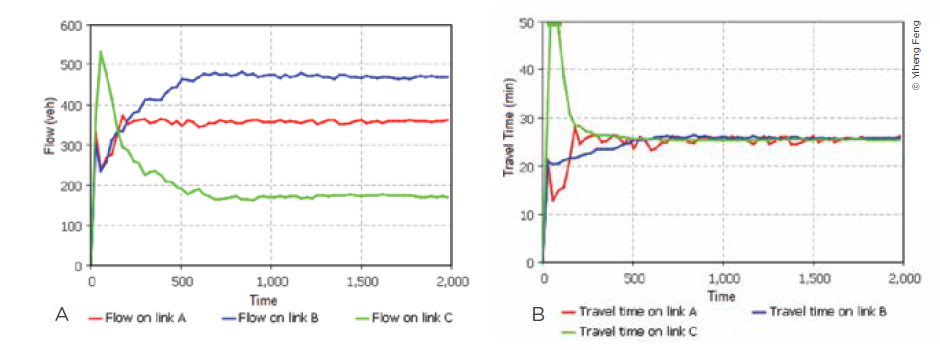
\includegraphics[scale=.75]{primer_results.png}
	\caption{Results of simulation from \cite{Zheng2013}}
	\label{fig:primer}
	\end{figure}

%%%%%%%%%%%%%%%%%%%%%%%%%%%%%%%%%%%%%%%%%%%%%%%%%%%%%%%%%%%%%%%%%%%%%%%%%%%%%%%%%
\subsection{Agent Rationality and Memory}
\cite{Wei2014} used AMBS to explore the effects rationality and memory to route choice behaviour.

They set out a model using reinforcement learning. With reinforcement learning, actions which lead to better outcomes are more likely to be repeated in the future, compared to actions that lead to worse outcomes. The reinforcement learning model they use is the Bush Mosteller (BM) model from literature \citep{Cross1973}. Under this model each action $c$ has a \textit{stimulus} $S_{c}^{i}$ on day $i$ given by equation \ref{eqn:BM}. $u_{c}$ is the payoff for action $c$ and $A_{i}$ desired payoff. The denominator represented the highest value of the $u_{c} - A_{i}$ over all actions $c$. Once the stimulus for each action is found, the probabilities of each action are updated by equation \ref{eqn:BMprob}, where $l$ is the learning rate. A higher $l$ allows the player to learn faster.

\begin{equation}
	S_{c}^{t} = \frac{u_{c} - A_{i} }{ \sup \left|u(k) - A_{i}\right|}
	\label{eqn:BM}
	\end{equation}

\begin{equation}
	p_{c}^{t+1}=\left\{\begin{array}{ll}
		p_{c}^{t}+\left(1-p_{c}^{t}\right) l s_{c}^{t}, & \text { if } s_{c}^{t} \geq 0 \\
		p_{c}^{t}+p_{c}^{t} l s_{c}^{t}, & \text { if } s_{c}^{t}<0
		\end{array}\right.
	\label{eqn:BMprob}
\end{equation}

They apply this to the traffic assignment problem using ABMS where each agent's actions are the different route choices available, using travel times as payoff. For the desired payoff, they use a weighted average of all the experienced travel times given by %equation \ref{eqn:ET}
\begin{equation*}
	A_{i}^{t}=\frac{\sum_{j=1}^{t-1} \psi^{t-1-j} T_{i}^{j}}{\sum_{j=1}^{t-1} \psi^{t-1-j}}
	\label{eqn:ET}
	\end{equation*}
for agent $i$ on day $t$. $T_{i}^{j}$ is the travel time on day $j$ and $\psi$ is the weighing parameter are represents the memory level. For the pay off of a given route $c$ they use %equation \ref{eqn:PT} then \ref{eqn:PT}
\begin{equation*}
	M_{i k}^{t}=\frac{\sum_{j=1}^{t} \psi^{t-j} T_{i}^{j} \xi_{i k}^{j}}{\sum_{j=1}^{t} \psi^{t-j} \zeta_{i k}^{j}}
	\label{eqn:PT}
	\end{equation*}
\begin{equation*}
	M_{i c}^{t}=\sum_{k=1}^{N} M_{i k}^{t} \xi_{i k}^{t}
	\label{eqn:PT2}
	\end{equation*}
 where $\xi = 1$ if path $k$ was taken on day $j$, else $\xi = 0$.

 By using these and \ref{eqn:BM} and \ref{eqn:BMprob} each agent can calculate the probabilities of choosing each route as $P_i = \{p^{i}_{1}, p^{i}_{2} ...\}$. A route is then selected when each agent generates a random number $b$ and chooses route $c$ by equation \ref{eqn:sumprob}
 \begin{equation}
	\sum_{j=1}^{c-1} p_{j}^{t}<b \leq \sum_{j=1}^{c} p_{j}^{t}
	\label{eqn:sumprob}
 \end{equation}

 They used this ABMS model on three test networks. Travel times are calculated with the BPR function in equation \ref{eqn:cap}. They explored the effects of the two key parameters: the learning rate $l$, and the memory level $\psi$.

 To explore $\psi$ they fixed $l = 0.3$ and tried $\psi = 0.1, 0.5, 0.9$. The results are shown in figure \ref{fig:reinf} lifted from their paper. For lower memory levels the flows fail to converge to the DUE, but instead fluctuate around it. The standard deviation of these flows decreases are $\psi$ increase. They note this makes sense as agents with better memory are able to make a better judgement. 

 \begin{figure}[h]
	\centering
	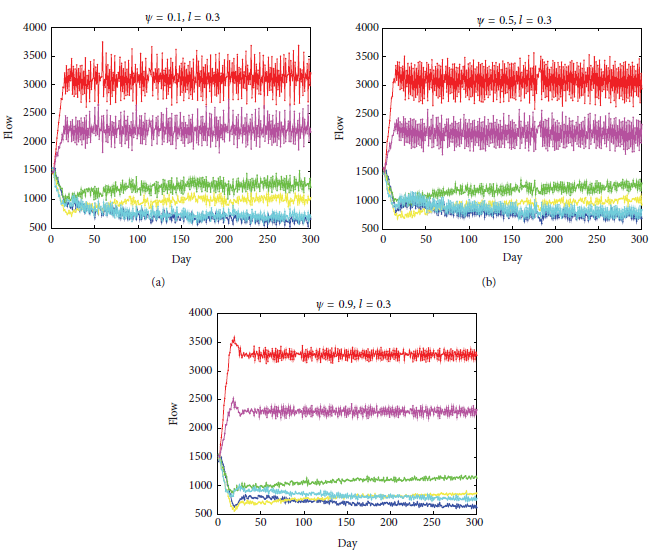
\includegraphics[scale=1]{reinf_paper.png}
	\caption{Effects of memory on stability from \cite{Wei2014}}
	\label{fig:reinf}
	\end{figure}

 To explore $l$ they then fixed $\psi = 0.6$ and tried $l = 0.1, 0.5, 0.9$. These results are shown in figure \ref{fig:reinf2} lifted from their paper. They only consider $l = 0.1$ to have converged while the other two did not. They note in the $l = 0.9$ case the flow converges to the DUE then leaves it again, and repeats that in a cycle. In the $l=.5$ case the flow fluctuates around different values to the DUE. They explain this behaviours by noting that a higher $l$ leads to faster change in the probabilities, leading to more variation. Lastly, they note a higher fixed $\psi$ slightly reduces the variation seen.

\begin{figure}[h]
	\centering
	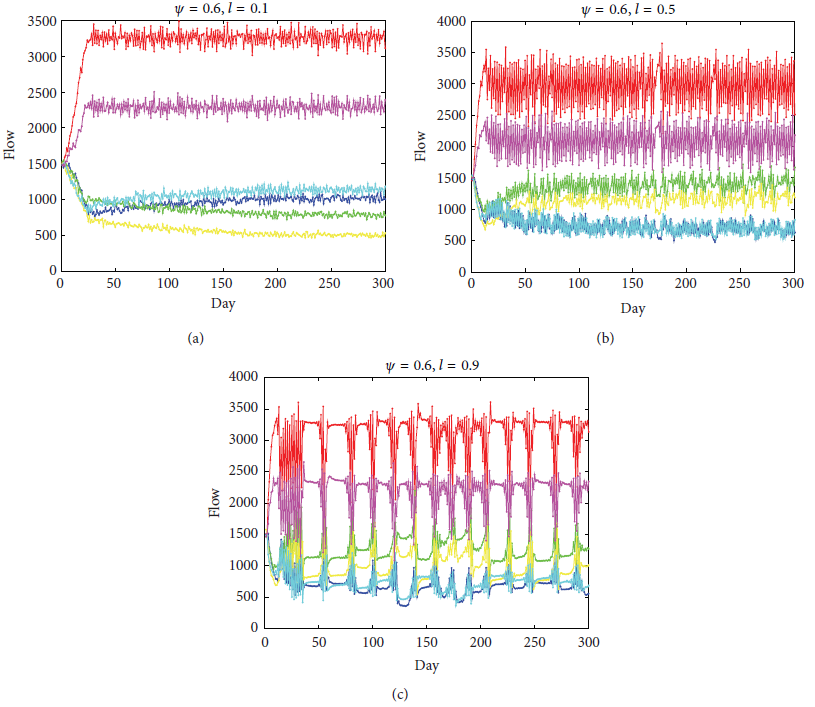
\includegraphics[scale=1]{reinf_paper2.png}
	\caption{Effects of learning rate on stability from \cite{Wei2014}}
	\label{fig:reinf2}
	\end{figure}

From this paper it can be seen that the intuitive idea that better memory and faster learning may not lead to stability. Irrationality may be important to stabilising flow on a network. 

%%%%%%%%%%%%%%%%%%%%%%%%%%%%%%%%%%%%%%%%%%%%%%%%%%%%%%%%%%%%%%%%%%%%%%%%%%%%%%%%%%%%%%%%%%%%%%%%%%%%%%%%%%
\subsection{Advanced Traveller Information Systems}
\cite{Liu2007} built an agent-based model on a small grid network, with an Advanced Traveller Information System (ATIS). The network had 9 nodes 12 links, and is displayed later in this report as Test Network 1, in figure \ref{fig:net1} with capacities and free flow in tables \ref{tab:net1}. The capacities mentioned in \ref{tab:net1} are double those use by \citeauthor{Liu2007}. Travel times are calculated with the BPR function again, given before in equation \ref{eqn:cap}.

They first solved a stochastic user equilibrium model, with the probabilities of each route given be a Gumbel distribution identical equation \ref{eqn:routeprobs}. They note on the parameter $\theta$ ``Higher is [$\theta$]-value, wiser drivers make route choice."" A higher $\theta$ value makes the fastest route more probable. They solve a convex minimisation problem on \ref{eqn:routeprobs} to find the equilibrium point. The results with different $\theta$ are shown in table \ref{tab:SUE} which is lifted from their paper, note in this table $\theta = \gamma$. The results show the flow along route $(1,4,7,8,9)$ converging to a value as the drivers become more rational, especially when $\gamma \geq 0.5$ 

\begin{table}[h!]
	\centering
	\caption{SUE results taken from \cite{Liu2007}}
	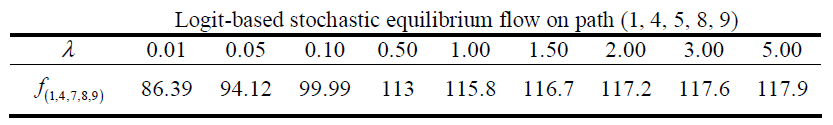
\includegraphics[scale=.75]{atis_tableSUE.png}
	\label{tab:SUE}
	\end{table}

Next they set up an ABMS model with an Advanced Traveller Information System. The ATIS allows drivers to look up the exact travel times, without perception error, on all routes from the previous day. Each agent weighs up this information with their perceived travel time on each route. Their new perceived travel times are given by equation \ref{eqn:atispaper} where agent $i$ on day $t+1$, for route $r$ and OD $w$, can look up the exact travel times $c_{r w}^{(i, t)}$ and mix them with their perceived travel times $\tau_{r w}^{(i, t)}$ with parameter $\alpha$.

When ATIS information is unreleased agents can only update perceived travel times on routes they have taken. They are able to weigh in day $n$ travel time  $c_{k w}^{(i, t)}$ with there expected travel time for the route $k \in R_k$ they chose, else they cannot update the travel time. This is shown in equation \ref{eqn:noatispaper}. In this case parameter $\beta$ is known as the learning rate.

\begin{equation}
	\tau_{r,w}^{(i, t+1)} = \alpha c_{r w}^{(i, t)} + (1-\alpha) \tau_{r w}^{(i, t)}; \alpha \in(0,1]
	\label{eqn:atispaper}
	\end{equation}

\begin{equation}
	\left\{\begin{array}{l}
	\hat{\tau}_{k w}^{(i, t+1)} = \beta c_{k w}^{(i, t)} + (1-\beta) \hat{\tau}_{k w}^{(i, t)}, \quad k \in R_{w}, \beta \in(0,1] \\
	\tau_{r w}^{(i, t+1)} = \tau_{r w}^{(i, t)}, \quad r \in R_{w}, r \neq k
	\end{array}\right.
	\label{eqn:noatispaper}
	\end{equation}

They ran a 2 simulation with 500 agents with OD node 1 to node 9. One simulation used an ATIS and one did not. The results are shown in table \ref{tab:atispaper} which is lifted from their paper. It can be seen that in both cases the flow converges to the equilibrium value from the SUE model, but it converges faster under the ATIS. However this behaviour breaks down as agents become too trusting of the ATIS. In figure \ref{fig:atisafig} lifted from their paper it can be seen that standard deviation of the flow along route $(1,4,7,8,9)$ increases with $\alpha$, and increases sharply for $\alpha \geq 0.25$. Too much trust in the ATIS leads to instability.

\begin{table}[h]
	\centering
	\caption{Simulation results taken from \cite{Liu2007}}
	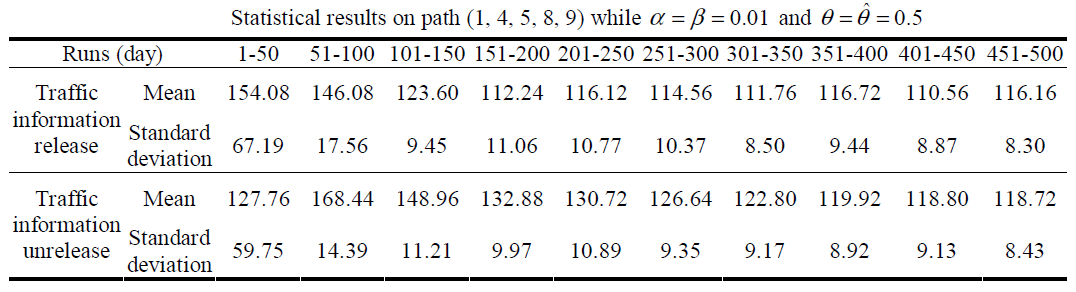
\includegraphics[scale=.7]{atis_table.png}
	\label{tab:atispaper}
	\end{table}

\begin{figure}[h]
	\centering
	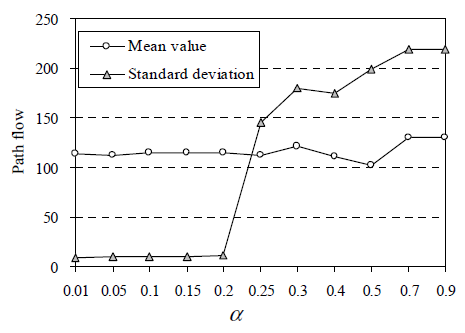
\includegraphics[scale=1]{atis_fig.png}
	\caption{Simulation results taken from \cite{Liu2007}}
	\label{fig:atisafig}
	\end{figure}

Their simulation results drew two key conclusions. Firstly, the system converged to the equilibrium predicted from a stochastic model faster when the ATIS system was used. Secondly, if the drivers put too much trust in that information the equilibrium becomes unstable.

%%%%%%%%%%%%%%%%%%%%%%%%%%%%%%%%%%%%%%%%%%%%%%%%%%%%%%%%%%%%%%%%%%%%%%%%%%%%%%%%%%%%%%%%%%%%%
\subsection{Route Choice Rules}
\cite{Nakayama2001} used ABMS to study the effects of heterogeneous route choice rules among different drivers. The 4 rules they explored were:

\begin{enumerate}
	\item{No switching}
	\item{Random switching}
	\item{Experience-only based switching}
	\item{Full rational switching}
	\end{enumerate}

Rules 1 and 2 are simple. Under rule 1 a driver never changes route after their initial selection and under rule 2 drivers choose a route without thinking, in a uniformly random manor. 

A driver using rule 3 only chooses a route based on experienced travel times according to equation \ref{eqn:routerule3}. Here $EC_{i,j}^{k}$ is the expected cost of route $j$ on day $i$, under rule $k$, $t^{\mathrm{avg}}\left(\mathbf{t}_{i j}, n_{i}^{k}\right)$ returns the average experience travel times over the last $n$ days, from set $\mathbf{t}_{i j}$, and $\gamma_{i}^{k}\left\{t^{\max }\left(\mathrm{t}_{i j}\right)-t^{\min }\left(\mathrm{t}_{i j}\right)\right\}$ captures the variability of travel times on route $j$, with $\gamma_{i}^{k}$ being the drivers' attitude to uncertainty. $k$ is included to label different formulations of this rule, each labelled with different $k$, having different $n$ and $\gamma$.

\begin{equation}
	EC_{i,j}^{k} = t^{\mathrm{avg}}\left(\mathbf{t}_{i j}, n_{i}^{k}\right) + \gamma_{i}^{k}\left\{t^{\max }\left(\mathrm{t}_{i j}\right)-t^{\min }\left(\mathrm{t}_{i j}\right)\right\}
	\label{eqn:routerule3}
	\end{equation}

A driver using rule 4 simply uses the average of all the travel times they have experienced on each route, choosing the smallest. Unlike in rule 3 where only the past $n$ days are considered, a rational rule 4 driver remembers all travel times.

Next they allow each agent in their simulation to change rule dynamically based on which rule is working best for them at that moment. Each rule $l$ has a performance indicator $f$ given by equation \ref{eqn:routeruleperf}, where $t_{i}$ is the travel time the agent experienced on day $i$ and $s$ is a parameters reflecting how much they learn from experience. Each driver chose the rule $l$ with minimal $f^{l}$ on day $i+1$.

\begin{equation}
	f_{i+1}^l = \left\{\begin{array}{ll}(1-s) f_{t}^{l} + s t_{i} & \text { if route used} \\ f_{i} & \text { otherwise }\end{array}\right.
	\label{eqn:routeruleperf}
	\end{equation}

The study ran an agent-based simulation on 4000 drivers on a network with 2 routes between the agents OD. Travel times were again calculated with the BPR in equation \ref{eqn:cap}, but the $0.15$ parameters and $4$ parameter are instead both $2$. Route 1 has capacity 4000 and free flow travel time 20, while route 2 has capacity 2000, and free flow 10. They solved

For their analysis, parameter $s=0.9$. Figure \ref{fig:routerules} shows the number of drivers that used each route choice rule, lifted from their paper. It can be seen that drivers did not converge to any rule and all four rules remained in use and somewhat stable. However travel times on all routes did stabilise to the times predicted using a deterministic user equilibrium.

\begin{figure}[h]
	\centering
	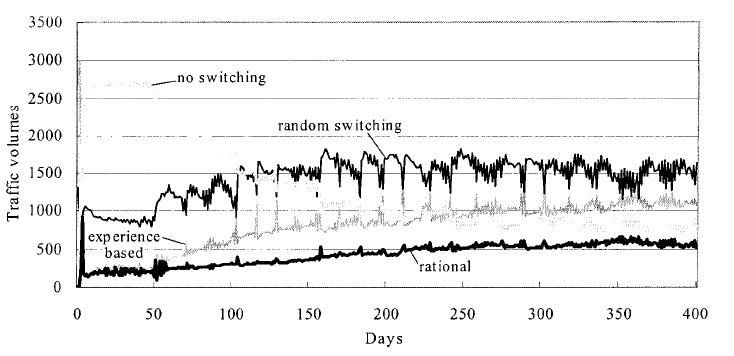
\includegraphics[scale=1]{route_rules.png}
	\caption{Simulation results taken from \cite{Nakayama2001}}
	\textit{The author was unable to find a colour copy of this figure with all four lines clearly visible.}
	\label{fig:routerules}
	\end{figure}

The finding of their paper do not fit with the assumption made by top-down models that all drivers are rational and homogeneous as all four rules remained in use through out the simulation, showing agents remained irrational with no incentive to learn to become rational. This contraction goes against classical models of network flow, and highlights the need for ABMS.

%%%%%%%%%%%%%%%%%%%%%%%%%%%%%%%%%%%%%%%%%%%%%%%%%%%%%%%%%%%%%%%%%%%%%%%%%%%%%%%%%%%%%%%%%%%%
\subsection{Autonomous Vehicles}
The challenge with route choice for autonomous vehicles is predicting interaction between human driven vehicles and AVs CITE(Li, Liu and Nie, 2018).

\cite{chen2017} looked into the road capacity on networks with both human and autonomous vehicles. They set out to build a systematic formulation of the operational capacity of roads and the effects of different AV penetrations. While their paper explores in detail the effects of dedicated AV lanes on roads, the content highlighted will focus on single-line mixed traffic, with AVs groups of traffic called \textit{platoons} of length $n$. 

They explore spacing between vehicles, based on the field test of CITE [Milanés et al., 2014; Shladover et al., 2010] and identify four spacing levels. The standard spacing is $S_0$, this represents the spacing, front bumper to front bumper, of regular HV traffic. They assume a HV will maintain at least the regular spacing behind an AV, so the spacing between an AV in front to a HV behind is $\beta^R s_0$ where $\beta^R \geq 1$. AVs travelling in a platoon of length $n$ will group closer together than normal HV traffic, as they are assumed to have faster reaction times thus needing a smaller safe distance to the vehicle ahead. As as results the spacing between AVs in a platoon is  $\gamma s_0$ where $\gamma < 1$. Lastly an AVs travelling behind a HV, or a different AV platoon will leave more space than is found within their platoon, so the spacing is $\beta^A s_0$ where $\beta^A \geq \gamma$. All these spacing are fixed and deterministic, and should be through of as long-term averages. Figure \ref{fig:avspacing} lifted from their paper shows all 4 levels of spacing, where $m$ is the average length of HC traffic. $\beta^R, \gamma $ and $\beta^A \geq 0$ 

\begin{figure}
	\centering
    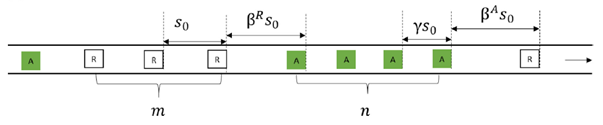
\includegraphics[scale=1]{av-spacing.png}
	\caption{Spacing of HVs and AVs from \cite{chen2017}}
	\label{fig:avspacing}
	\end{figure}

From these spacings, they find the average spacing as
$$
\bar{S} = \frac{\beta^{A} S_{0} + (n-1) \gamma S_{0} + \tilde{m}\left(\beta^{R} S_{0} + (m-1) S_{0}\right)}{n+m}
$$
where $\tilde{m}$ is 1 when $m > 0$ and 0 when $m = 0$, to indicate whether HVs are present. Even when $m=0$ AVs will not form into one continuous platoon as it is assumed platooning requires communications between vehicles, which is only possible over a finite range. From this they define the \textit{av gain} $\varepsilon$ as given by equation \ref{eqn:avgain} where $\alpha$ is the proportion of AVs to the total traffic.

\begin{equation}
	\varepsilon = \left\{\begin{array}{ll}
		1 - \gamma - \left(\frac{\beta^{A}-\gamma}{n} + \frac{\beta^{R}-1}{n}\right), & \text { if } 0 \leq \alpha<1 \\
		1-\gamma-\frac{\beta^{A}-\gamma}{n}, & \text { if } \alpha=1
		\end{array}\right.
	\label{eqn:avgain}
	\end{equation}

Note as $\beta^R \geq 1, \gamma < 1$ and $\beta^A \geq \gamma$, $\varepsilon < 1$. Using equation \ref{eqn:avgain} the average spacing can be rewritten as
$$
\bar{S} = S_0 (1 - \alpha \varepsilon)
$$
so it is clear that a higher $\alpha$ leads to smaller average spacings. \citeauthor{chen2017} then use this to derive the capacity as a function of $\alpha$ and $\varepsilon$ stating that, when $C_0$ is the capacity of a road under just HV traffic, with AVs and HVs the capacity is adjusted by equation \ref{eqn:capgain}.

\begin{equation}
	C = f(\alpha, \varepsilon) = \frac{C_0}{1 - \alpha \varepsilon} 	
	\label{eqn:capgain}
	\end{equation}

From equation \ref{eqn:capgain} they derive four intuitive rules:

\begin{itemize}
	\item Capacity increases with platoon size $n$
	\item Capacity decreases with $\gamma$
	\item Capacity decreases with $\beta^A$
	\item Capacity increases with AV proportion $\alpha$ at an increasing rate.
	\end{itemize}

From this work it is clear and AMBS using mixed HV/AV traffic would need to consider link capacity as a function of the proportion of AVs in the traffic, and the AV gain, defined by setting values for the spacing parameters.

%%%%%%%%%%%%%%%%%%%%%%%%%%%%%%%%%%%%%%%%%%%%%%%%%%%%%%%%%%%%%%%%%%%%%%%%%%%%%%%%%%%%%%%
\subsection{Conclusions and Research Opportunities}
Methods exist to tackle the traffic assignment problem, from the early DUEs of Wardrop to the SUEs of Daganzo and Sheffi and Cascetta. However these homogeneous models fail in that they assume drivers to be rational, which isn't the case as is shown by the work of \cite{Nakayama2001} where driver-agents did not become rational when learning how to choose a route. It is for this reason that agent based modelling and simulation has emerged as the contemporary approach to modelling traffic flow, and this method will be used in this report. The case for ABMS is made well in the primer by \cite{Zheng2013}.

The work of \cite{Liu2007} raises an import concern when thinking about autonomous vehicles. Too much trust in an advanced traveller information system, through which drivers can look up past travel times on any route, leads to instability. It is reasonable to assume that all agents simply see the fastest route, and all choose it, causing heavy traffic and slowing the route down. Autonomous vehicles will have access to much better information than humans, so maintaining heterogeneous decision making will be vital to evenly distributing traffic to minimise travel times. 

Lastly it is clear from the work of \cite{chen2017} that links behave differently with mixed traffic than with human traffic. Autonomous vehicles lead to high capacities which should reduce travel times. However the highlighted work did not explore this effect with ABMS.

An few areas of research emerge from this literature review. Most obviously is the need for AMBS of day to day traffic demand and flow dynamics with mixed human and autonomous vehicles on which there has been little research compared to the human-only case. However the rationality of autonomous vehicles should be explored, especially the idea of making them irrational like a human. The rationality of the human traffic and the effect this has on the overall mixed traffic is also work exploring. 

The goal of this report is therefore to explore with ABMS day to day traffic demand and flow dynamics with mixed human and autonomous vehicles, and the effects of information and rationality.

\pagebreak
%%%%%%%%%%%%%%%%%%%%%%%%%%%%%%%%%%%%%%%%%%%%%%%%%%%%%%%%%%%%%%%%%%%%%%%%
% Method
%%%%%%%%%%%%%%%%%%%%%%%%%%%%%%%%%%%%%%%%%%%%%%%%%%%%%%%%%%%%%%%%%%%%%%%%

\section{Methodology/ The Model}
\subsection{Overview}
It is assumed that a number of vehicles $N$ wish to travel on a road network. These vehicles may use human driven or autonomous, the number of each is given by $N_{hv}$ and $N_{av}$ for HVs and AVs respectively, and $N_{hv} + N_{av} = N$. Each vehicle is an independent agent. Each agent has separate knowledge of travel times, an origin and destination between which they want to travel, and choose their route independently of other agents. This constitutes each agent's belief, desire, and intention.

The simulation allows all $N$ agents to make their journey on a given network. On one day each agent travels from their origin to their destination. Within-day dynamics is not considered, travel times assume all agents that travel on a road do so simultaneously. This assumption makes modelling easier, and is suitable for simulating events such as rush-hour when many drivers take to the roads on their daily commute.

Each agent has a degree of rationality, represented as preference towards their perceived shortest route. Each driver is also able to look up the previous day's travel times on any route using the ATIS, and can trust it as much as they want. Error terms are also used on perceived travel times for a route they have travel. It is assumed AVs are more rational than HVs, have better memory, and update their memory on all routes available at the end of the day, while HVs only update travel times they actually experience, thus only the route they travel on.

At the start of the day, each driver chooses a route randomly. There is a fixed probability $\beta$ of them deciding to try a new route today, if so then the probability of each alternative route is a function of their perceived travel times on each of the routes, such that faster routes are preferred. Perceived travel times balance both memory and ATIS information. The rationality parameter $\theta$ controls the distribution, higher thetas make the shortest route more likely. Once all agents have picked a route, the numbers are counted per link so that travel times can be calculated. Busy links lead to slower travel times.

At the end of the day each agent adjusts its memory. HVs update their list of remembered travel times for each link they travelled on, with error. AVs update for all links in the network as they have access to better information, there is error on this too but by default it is 0. It is now possible to run the simulation again for another day.

The parameters in the model, with their default values, are shown in table \ref{tab:params}. These values can be varied to study their effects.

\begin{table}[h!]
	\begin{center}
		\caption{Model parameters and default values}
		\label{tab:params}
		\begin{tabular}{c|c|l}
			\hline
			Parameter & Default Value & Description \\
			\hline
			$D$ & $500$ & The number of days the simulation is ran for\\
			$N_{hv}, N_{av}$ & $500, 500$ & The number of HVs and AVs \\
			& & respectively\\
			$e_{hv}, e_{av}$ & $5,0$ & The standard deviation error in perceived travel times for \\
			& & HVs and AVs respectively. Errors are normal  \\
			& & random variables with mean 0\\
			$L_{hv}, L_{av}$ & $3, 1000$ & the memory length in days for HVs and AVs respectively\\
			$\theta_{hv}, \theta_{av} $ & $ 0.5, 1 $ & The rationality of HVs and AVs respectively\\
			$\alpha_{hv}, \alpha_{av}$ & $0, 0 $ & The ATIS bias of HVs and AVs respectively\\
			$\beta$ & 0.5 & The probability of a HV choosing a new route on a given \\ 
			& &  day. There is not such value for AVs which always \\ 
			& &  consider all routes\\
			\hline
			\end{tabular}
		\end{center}
	\end{table}

When choosing a new route, the probability for agent $i$ choosing route $j$, with given $\theta$, and $\beta$ is given by equation \ref{eqn:prob}. Note for an AV, $\beta = 1$. The probability of \textit{not} changing route, and using the same as yesterday is $1-\beta$ for HVs. This is the Gumbel distribution often used in literature such as \cite{Zheng2013} and \cite{Liu2007}.

\begin{equation}
	p_{i,j}(d) = \beta \frac{\exp \left(-\theta t_{i, j}\right)}{\sum_{k} \exp \left(-\theta t_{i, k}\right)}
	\label{eqn:prob}
	\end{equation}

$t_{i, j}$ is the perceived travel time of that route, given by the average of the the agents memory $m_{j}$, mixed with ATIS information giving the exact travel times from the previous day $c_{j}$, and is given in equation \ref{eqn:atis}. This equation is based of \cite{Liu2007}.

\begin{equation}
	t_{i, j} = \alpha m_{j} + (1-\alpha) c_{j}
	\label{eqn:atis}
	\end{equation}

The travel time $c_{l}$ on each link $l$ is a function of the links traffic count $v_{l}$, capacity $Y_{l}$, and free-flow travel time $c_{l}^{0}$ (the travel time with no traffic) given in equation \ref{eqn:cap}, the BPR function used through literature.

\begin{equation}
	c_{l} = c_{l}^{0}( 1 + 0.15(v_{l}/Y_{l})^{4})
	\tag{\ref{eqn:cap}}
	\end{equation}

However as the capacity of a link increases with the proportion of AVs to AVs + HVs, $Y_{l}$ is a function of $N_{hv}$ and $N_{av}$ given in equation %\ref{eqn:capgain2}.

\begin{equation}
	Y_{l} = f (\alpha, \varepsilon) = \frac{Y_{l,0}}{1 - \alpha \varepsilon} 
	\label{eqn:capgain2}
	\end{equation}
where
\begin{equation}
	\alpha = \frac{ N_{av}	}{ N_{hv} + N_{av} }
	\label{eqn:avprop}
	\end{equation}
and
\begin{equation}
	\varepsilon = \left\{\begin{array}{ll}
		1 - \gamma - \left(\frac{\beta^{A}-\gamma}{n} + \frac{\beta^{R}-1}{n}\right), & \text { if } 0 \leq \alpha<1 \\
		1-\gamma-\frac{\beta^{A}-\gamma}{n}, & \text { if } \alpha=1
		\end{array}\right.
	\label{eqn:avgain2}
	\end{equation}

The constraints on $\gamma, \beta^{A}$ and $\beta^{R}$ are $\beta^R \geq 1, \gamma < 1, \beta^A \geq \gamma$, $\varepsilon < 1$, and $\beta^R,  \gamma, \beta^A \geq 0$. Under these constraints, the values chosen are $\beta^A = 0.9, \beta^R = 1.2, \gamma = 0.75$. The platoon length $n=5$ is used.


\subsection{Program}
The simulation is written in python, with classes for HVs, AVs, links, and networks. The simulation ran in a Jupyter Lab interactive environment, with class and function definitions in imported modules. The program is structured as follows.

\begin{enumerate}
	\item Global initialisation: set values for the model parameters.
	\item Define a list of links, with a start, end, capacity, and free flow travel time.
	\item Define a network from this list of links. 
	\item Define a list of agents, HVs and AVs each with an origin and destination.
	\item Simulate day 1. Each agent has a method to run on day 1. Their OD is sent to the network to get all available routes, their memory is initialised as the free flow travel time, plus a large random error, given by 10 times their normal error standard deviation. They then pick a route.
	\item The network updates. Counts per links are made and travel times are calculated.
	\item Data is saved on the counts per link and per route, using the state of the network, and by looping through all agents and recording their route.
	\item The drivers amend their memory. HVs remember up to $L_{hv}$ travel times per link and add their experienced travel time plus error for each link from the previous trip to their memory. AVs do the same but for all links. They then pick a new route.
	\item Loop through 6,7,8 for $D$ Days.
	\end{enumerate}

The program is coded in an object orientated manor, with the network object built from link objects. This makes the model versatile and it can be quickly applied to any network. Link objects contain a method to calculate travel times, with capacity adjustment depending on the number of AVs using the link. The network object contains methods to find all paths between an origin and destination, and a method to count how many agents used each link then calculate travel times with each links travel time method.

The main limitations of this program are: the path finding algorithm used only works on finite acyclic digraphs (no loops or infinite paths allowed); and if links are significantly over capacity, thus travel times are high enough, the denominator of equation \ref{eqn:prob} used when agents pick a route may come out as zero due to finite resolution, crashing the simulation. Two prevent the second limitation from happening, the total capacity of the network between any OD is not lower than the number of agents.

\subsection{Usage}
The model was used to run simulations with varied initialisation parameters to study their effects. The simulations ran are listed below. All other variables are held at their default values.

\begin{itemize}
	\item $(N_{hv}, N_{av}) = (1000,0), (900,100), ... (100, 900), (0, 1000)$ 
	\item $\theta_{hv} = 0.01, 0.05, 0.1, .2, .3, .4, .5, 1, 2, 3$ 
	\item $\theta_{av} = 0.01, 0.05, 0.1, .2, .3, .4, .5, 1, 2, 3$
	\item $ L_{hv} = 1, 2, 3, 4 , 10, 30, 50, 100, 250$
	\item $ L_{av} = 1, 2, 3, 4 , 10, 30, 50, 100, 250$
	\item $ \alpha_{hv},\alpha_{hv} = (0,0) , (0,.5) ,(0.5,0), (.5,.5) $
	\end{itemize}

For each simulation, route count data per day was saved to a file. These datasets were analysed in a separate notebook.

The first network used for analysis is Test Network 1, shown in figure \ref{fig:net1}, with capacities and free flow travel times in table \ref{tab:net1}. All agents on this network wish to travel from node 1 to node 9, there are 6 possible paths for this, labelled route 0 to route 5 and detailed in table \ref{tab:net1routes}. This network is taken from Wei et al.'s paper \cite{Wei2014}, with the only difference being each capacity is doubled.

\newpage
\begin{figure}[h!]
	\centering
	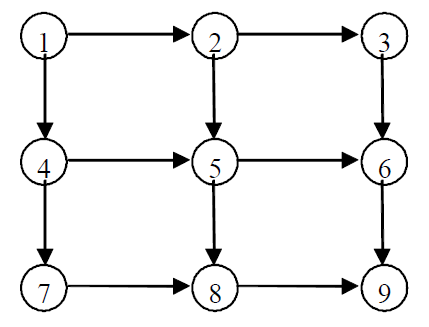
\includegraphics[scale=.75]{net1.png}
	\caption{Nodes and links in Test Network 1}
	\label{fig:net1}
	\end{figure}

\begin{table}[h!]
	\begin{center}
		\caption{Capacities and free flow travel times in Test Network 1}
		\label{tab:net1}
		\begin{tabular}{ccc|ccc}
			\hline 
			Link & $C_{l}^{0}$ & $Y_{l}$ & Link & $C_{l}^{0}$ & $Y_{l}$ \\
			\hline
			(1-2) & 20 & 720 & (5-6) & 12 & 360 \\
			(2-3) & 12 & 720 & (4-7) & 15 & 480 \\
			(1-4) & 15 & 480 & (58) & 10 & 300 \\
			(2-5) & 12 & 360 & (6-9) & 30 & 720\\
			(3-6) & 12 & 720 & (7-8) & 15 & 480 \\
			(4-5) & 10 & 300 & (8-9) & 15 & 480 \\
			\hline
			\end{tabular}
		\end{center}
	\end{table}

\begin{table}[h!]
	\begin{center}
		\caption{Paths between nodes 0 and 9 in Test Network 1.}
		\label{tab:net1routes}
		\begin{tabular}{c|c}
			\hline
			Path & Links \\
			\hline
			Route 0 & (1-2), (2-3), (3-6), (6-9)\\
			Route 1 & (1-2), (2-5), (5-6), (6-9)\\
			Route 2 & (1-2), (2-5), (5-8), (8-9)\\
			Route 3 & (1-4), (4-5), (5-6), (6-9)\\
			Route 4 & (1-4), (4-5), (5-8), (8-9)\\
			Route 5 & (1-4), (4-7), (7-8), (8-9)\\
			\hline
			\end{tabular}
		\end{center}
	\end{table}


\pagebreak
%%%%%%%%%%%%%%%%%%%%%%%%%%%%%%%%%%%%%%%%%%%%%%%%%%%%%%%%%%%%%%%%%%%%%%%%
% Results
%%%%%%%%%%%%%%%%%%%%%%%%%%%%%%%%%%%%%%%%%%%%%%%%%%%%%%%%%%%%%%%%%%%%%%%%

\section{Results}

\subsection{Default Simulation}
The simulation was ran on Test Network 1 with all the default parameters to access its performance and behaviour. All agents travelled for node 1 to node 9 for 500 days, the number of agents choosing each route is recorded each day and plotted in figure \ref{fig:defaults}. By taking the mean of the last 250 days, it is possible to estimate the converge point for each route, these means are shown in table \ref{tab:defaultcov} and marked with black dashed lines in figure \ref{fig:defaults}. In figure \ref{fig:defaults_tts} the travel time for each route are shown over the course of the simulation and the average travel times for the last 250 days are also show in table \ref{tab:defaultcov}. This simulation was ran multiple times and these results can be considered typical.

\begin{table}[h!]
	\begin{center}
		\caption{Apparent point of converge for each route on Test Network 1}
		\label{tab:defaultcov}
		\begin{tabular}{c|c|c}
			\hline
			 & \multicolumn{2}{c}{Mean: last 250 days}\\
			Path & Traffic Flow & Travel Time \\
			\hline
			Route 0 & 305.2 & 85.4\\
			Route 1 & 112.1 & 87.7\\
			Route 2 & 123.4 & 86.3\\
			Route 3 & 74.9 & 87.2\\
			Route 4 & 172.3 & 85.8\\
			Route 5 & 212.1 & 86.0\\
		
			\hline
			\end{tabular}
		\end{center}
	\end{table}



%%%%%%%%%%%%%%%%%%%%%%%%%%%%%%%%%%%%%%%%%%%%%%%%%%%%%%%%%%%%%%%%%%%%%%%%%%%%%%%%%%%%%%
\subsection{Effects of AV Proportion}
To study the effects of the proportion of AVs to HVs, eleven simulations where ran varying the amount of each, with $(N_{hv}, N_{av}) = (1000,0), (900,100), ... (100, 900), (0, 1000)$.
To visualise the data, two figures are drawn. Figure \ref{fig:Nhvavgrid} shows a sample of four simulations with traffic on routes 0 and 2 displayed. Figure \ref{fig:Nhvav} shows the standard deviation of traffic flow per route over the previous five days, for each simulation ran. This gives measure of stability around the convergence values. Each route converged to approximately the same values as the default run. 

\begin{figure}[h!]
	\centering
	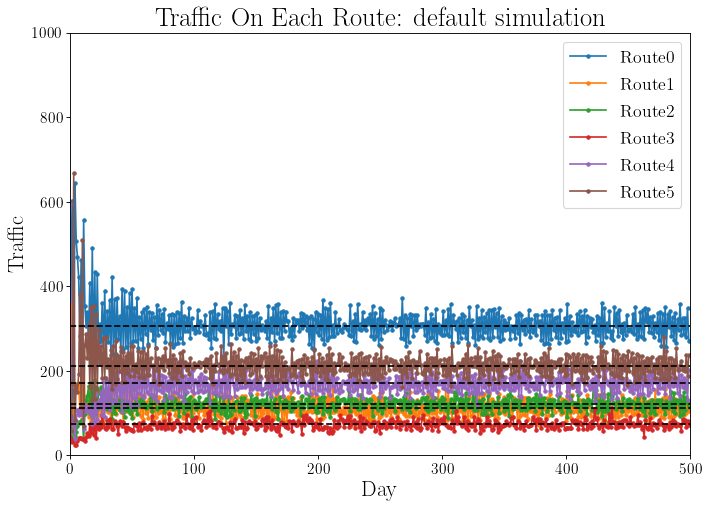
\includegraphics[scale=.5]{default.png}
	\caption{Simulation results from default parameters}
	\label{fig:defaults}
	\end{figure}

\begin{figure}[h!]
	\centering
	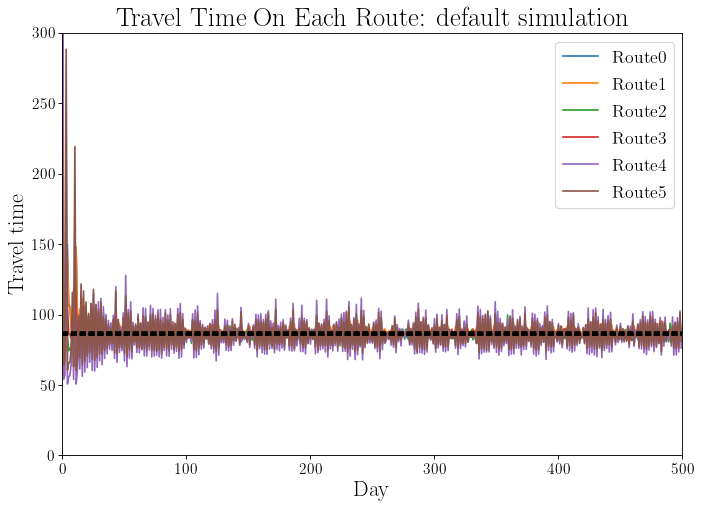
\includegraphics[scale=.5]{default_tts.png}
	\caption{Route Travel times with default parameters}
	\label{fig:defaults_tts}
	\end{figure}

\begin{figure}[h!]
	\centering
	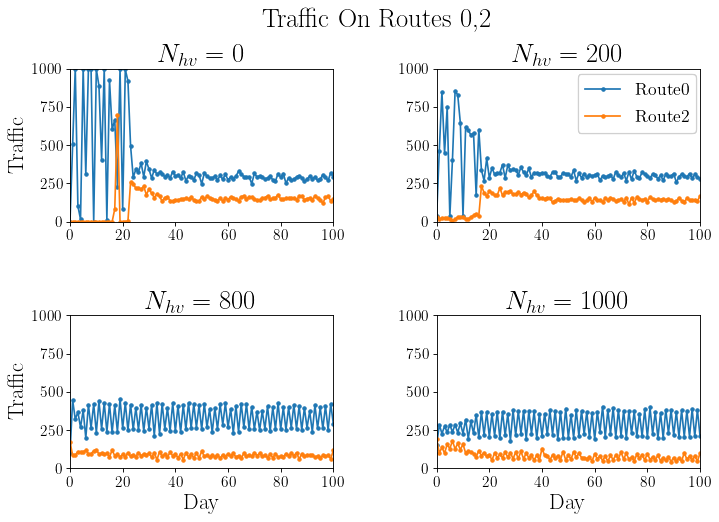
\includegraphics[scale=.5]{hv_vs_av_grid.png}
	\caption{Results of simulations with different $N_{av},N_{hv}$}
	\label{fig:Nhvavgrid}
	\end{figure}

\begin{figure}[h!]
	\centering
	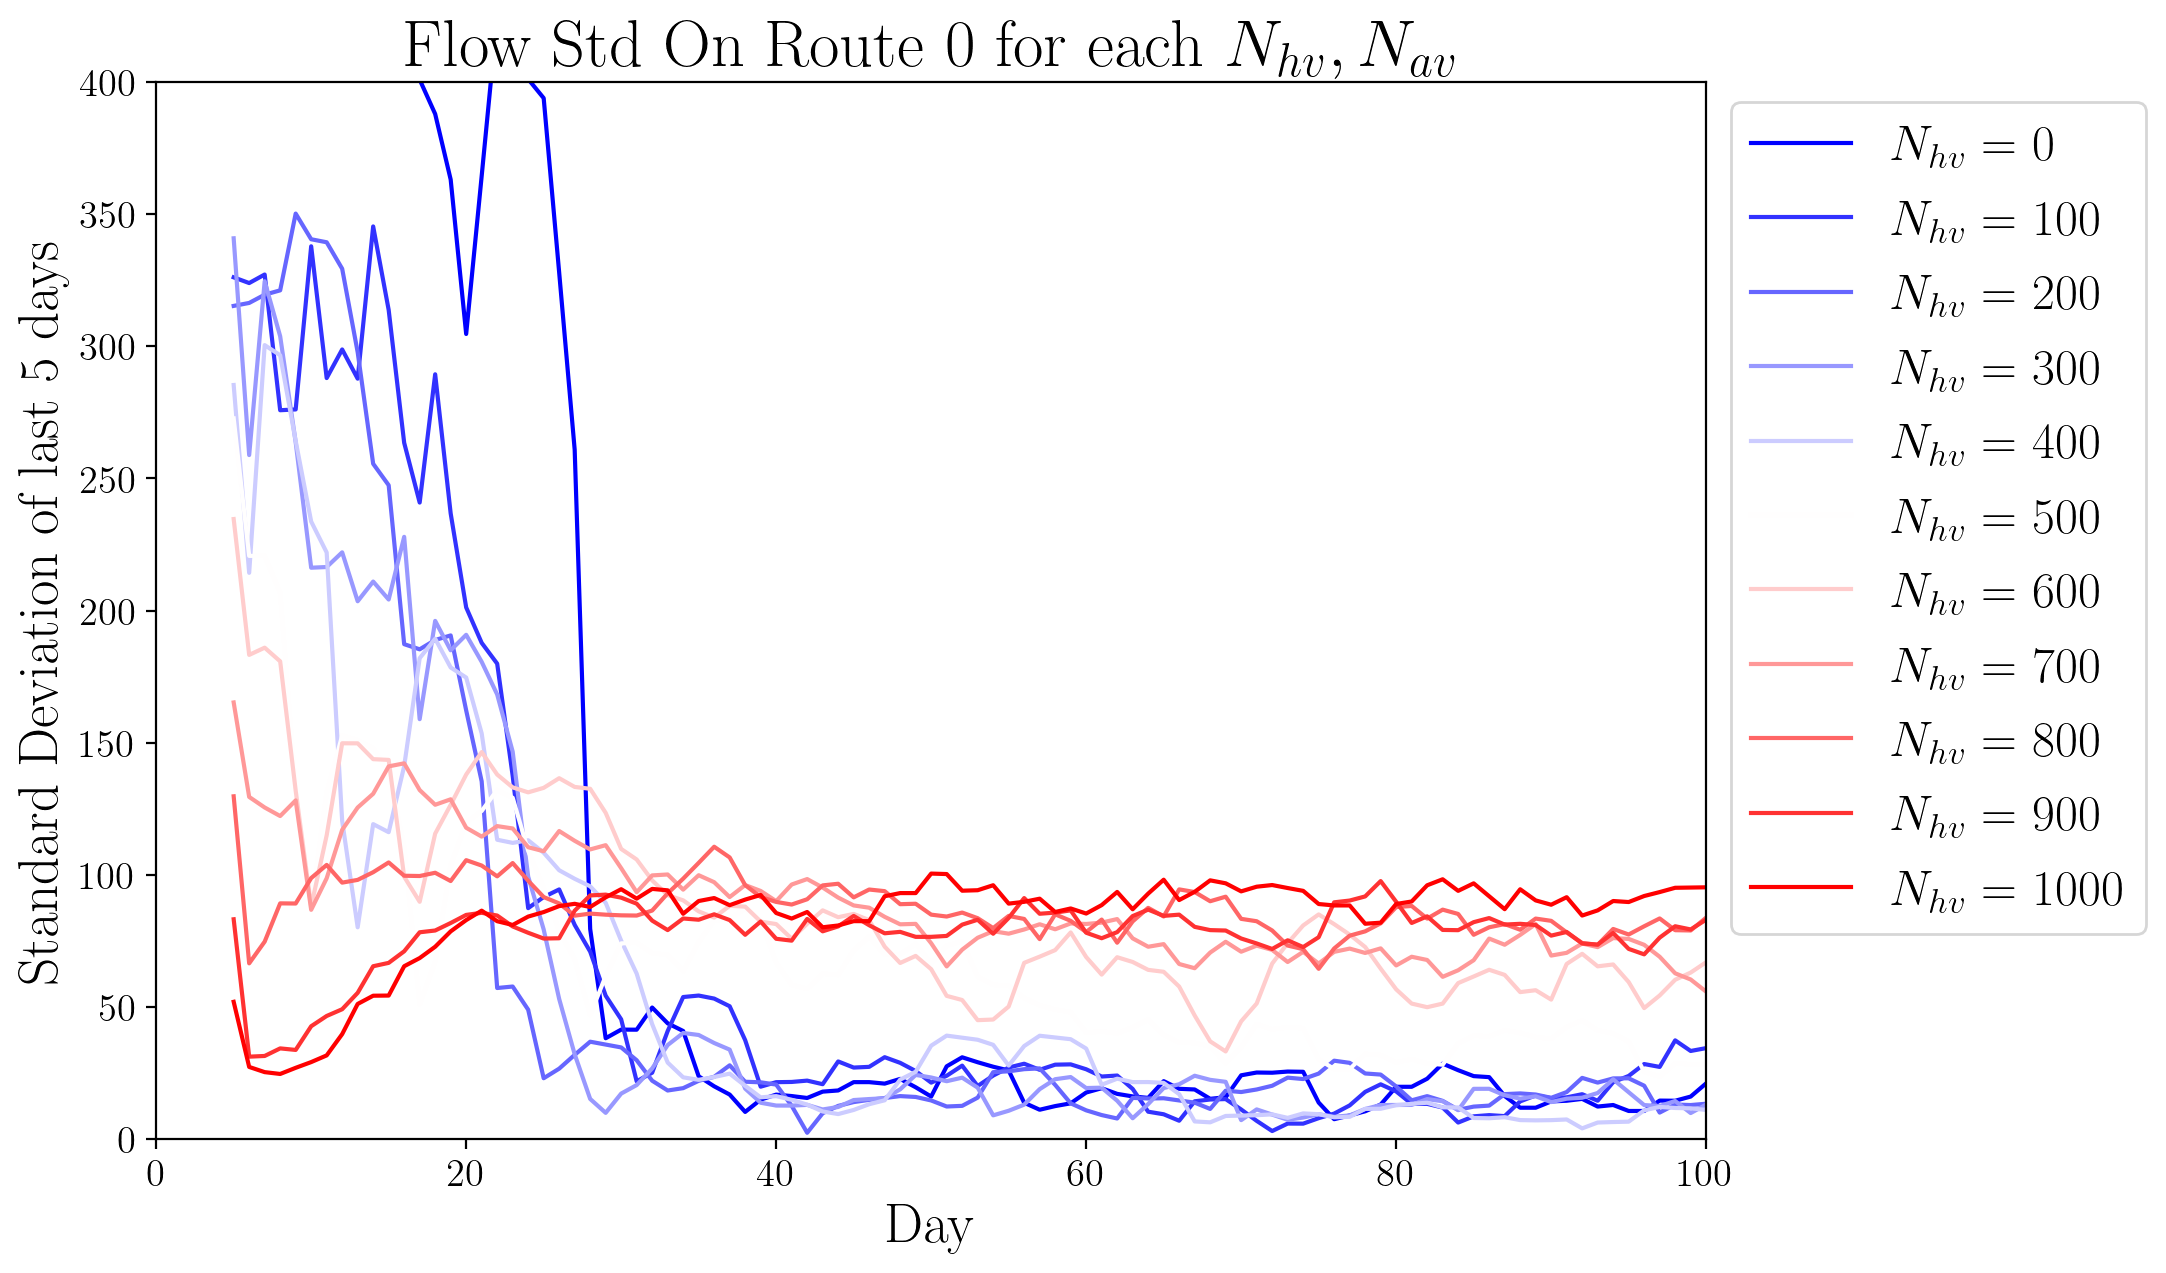
\includegraphics[scale=.5]{hv_av_std.png}
	\caption{Results of simulations with different $N_{av},N_{hv}$}
	\label{fig:Nhvav}
	\end{figure}


\subsection{Effects of $\theta_{hv}$}
The simulation was ran 10 times with default parameters but varying $\theta_{hv}$ through
$$0.01, 0.05, 0.1, 0.2, 0.3, 0.4, 0.5, 1, 2, 3$$
In figure \ref{fig:hvthgrid}, four simulations are shown for references, with the traffic on routes 0 and 2 shown over the course of the simulation. In figure \ref{fig:hvthstd} the 5 day standard deviation is shown for each $\theta_{hv}$ value.

\begin{figure}[h!]
	\centering
	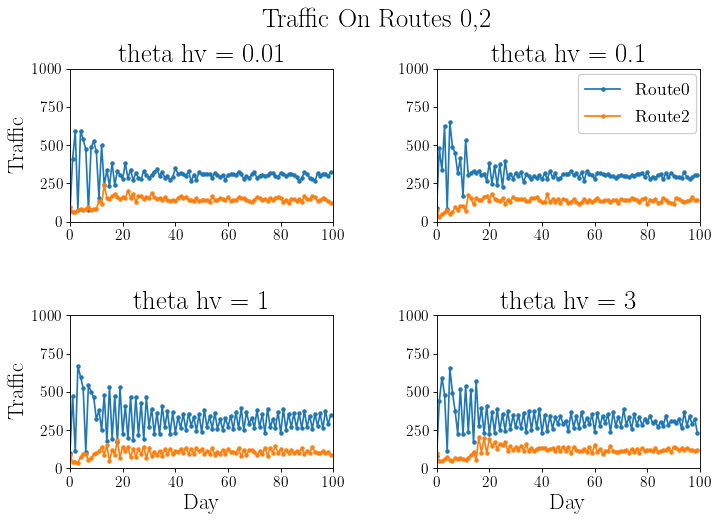
\includegraphics[scale=.5]{hv_th_grid.png}
	\caption{Results of simulations with different $\theta_{hv}$}
	\label{fig:hvthgrid}
	\end{figure}

\begin{figure}[h!]
	\centering
	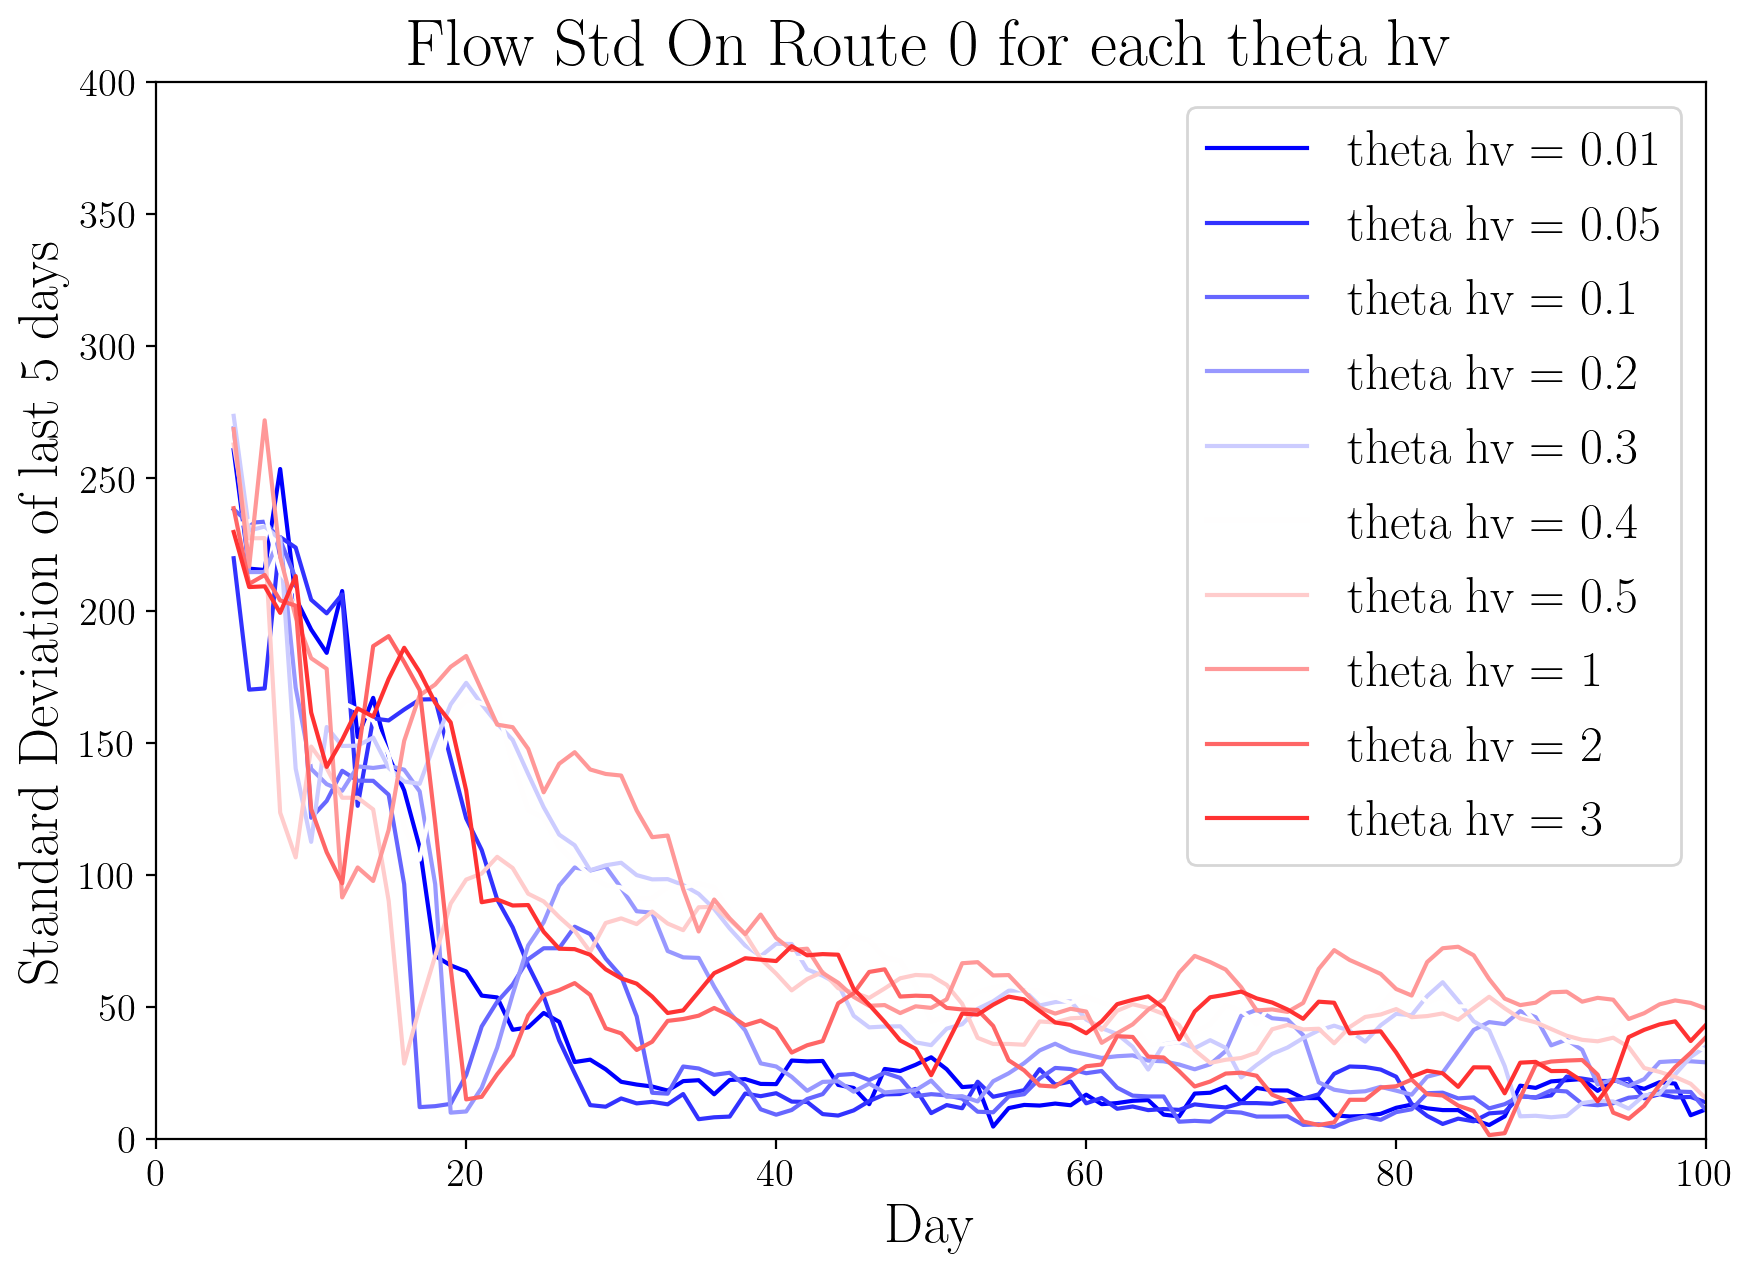
\includegraphics[scale=.5]{hv_th_std.png}
	\caption{Results of simulations with different $\theta_{hv}$}
	\label{fig:hvthstd}
	\end{figure}

%%%%%%%%%%%%%%%%%%%%%%%%%%%%%%%%%%%%%%%%%%%%%%%%%%%%%%%%%%%%%%%%%%%%%%%%%%%%%%
\subsection{Effects of $\theta_{av}$}
The simulation was ran 10 times with default parameters but varying $\theta_{av}$ through
$$0.01, 0.05, 0.1, 0.2, 0.3, 0.4, 0.5, 1, 2, 3$$
In figure \ref{fig:avthgrid}, four simulations are shown for references, with the traffic on routes 0 and 2 shown over the course of the simulation. In figure \ref{fig:avthstd} the 5 day standard deviation is shown for each $\theta_{av}$ value. Figure \ref{fig:avth3001}, the traffic on route 0 is shown in detail for $\theta_{av} = 0.01, 3$.

\begin{figure}[h!]
	\centering
	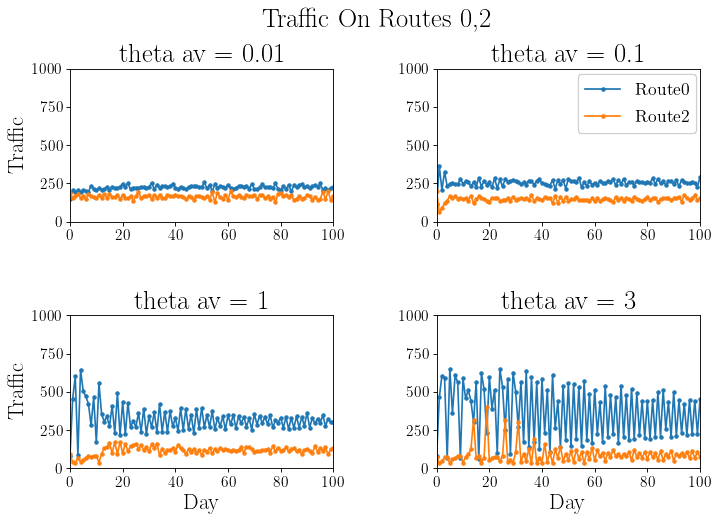
\includegraphics[scale=.5]{av_th_grid.png}
	\caption{Results of simulations with different $\theta_{av}$}
	\label{fig:avthgrid}
	\end{figure}

\begin{figure}[h!]
	\centering
	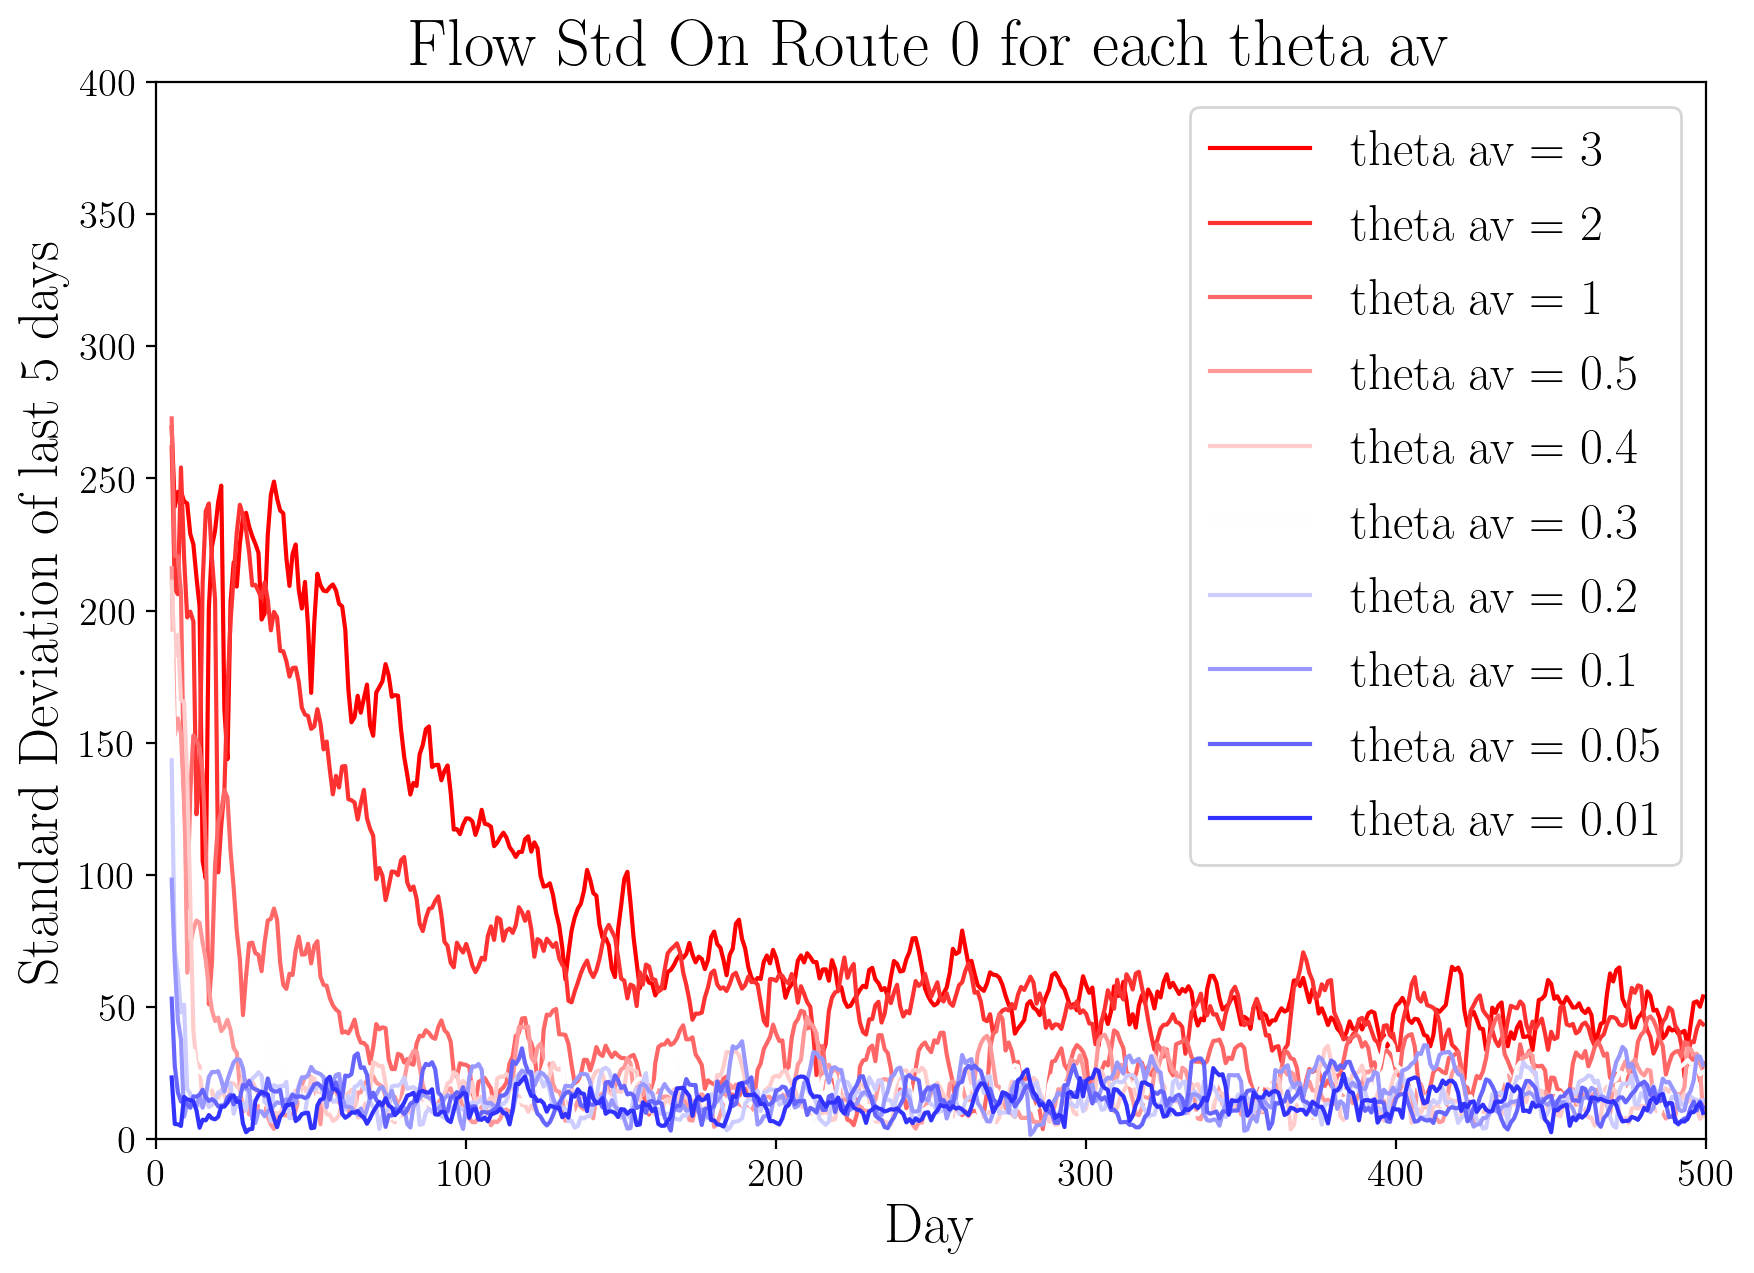
\includegraphics[scale=.5]{av_th_std.png}
	\caption{Results of simulations with different $\theta_{av}$}
	\label{fig:avthstd}
	\end{figure}

\begin{figure}[h!]
	\centering
	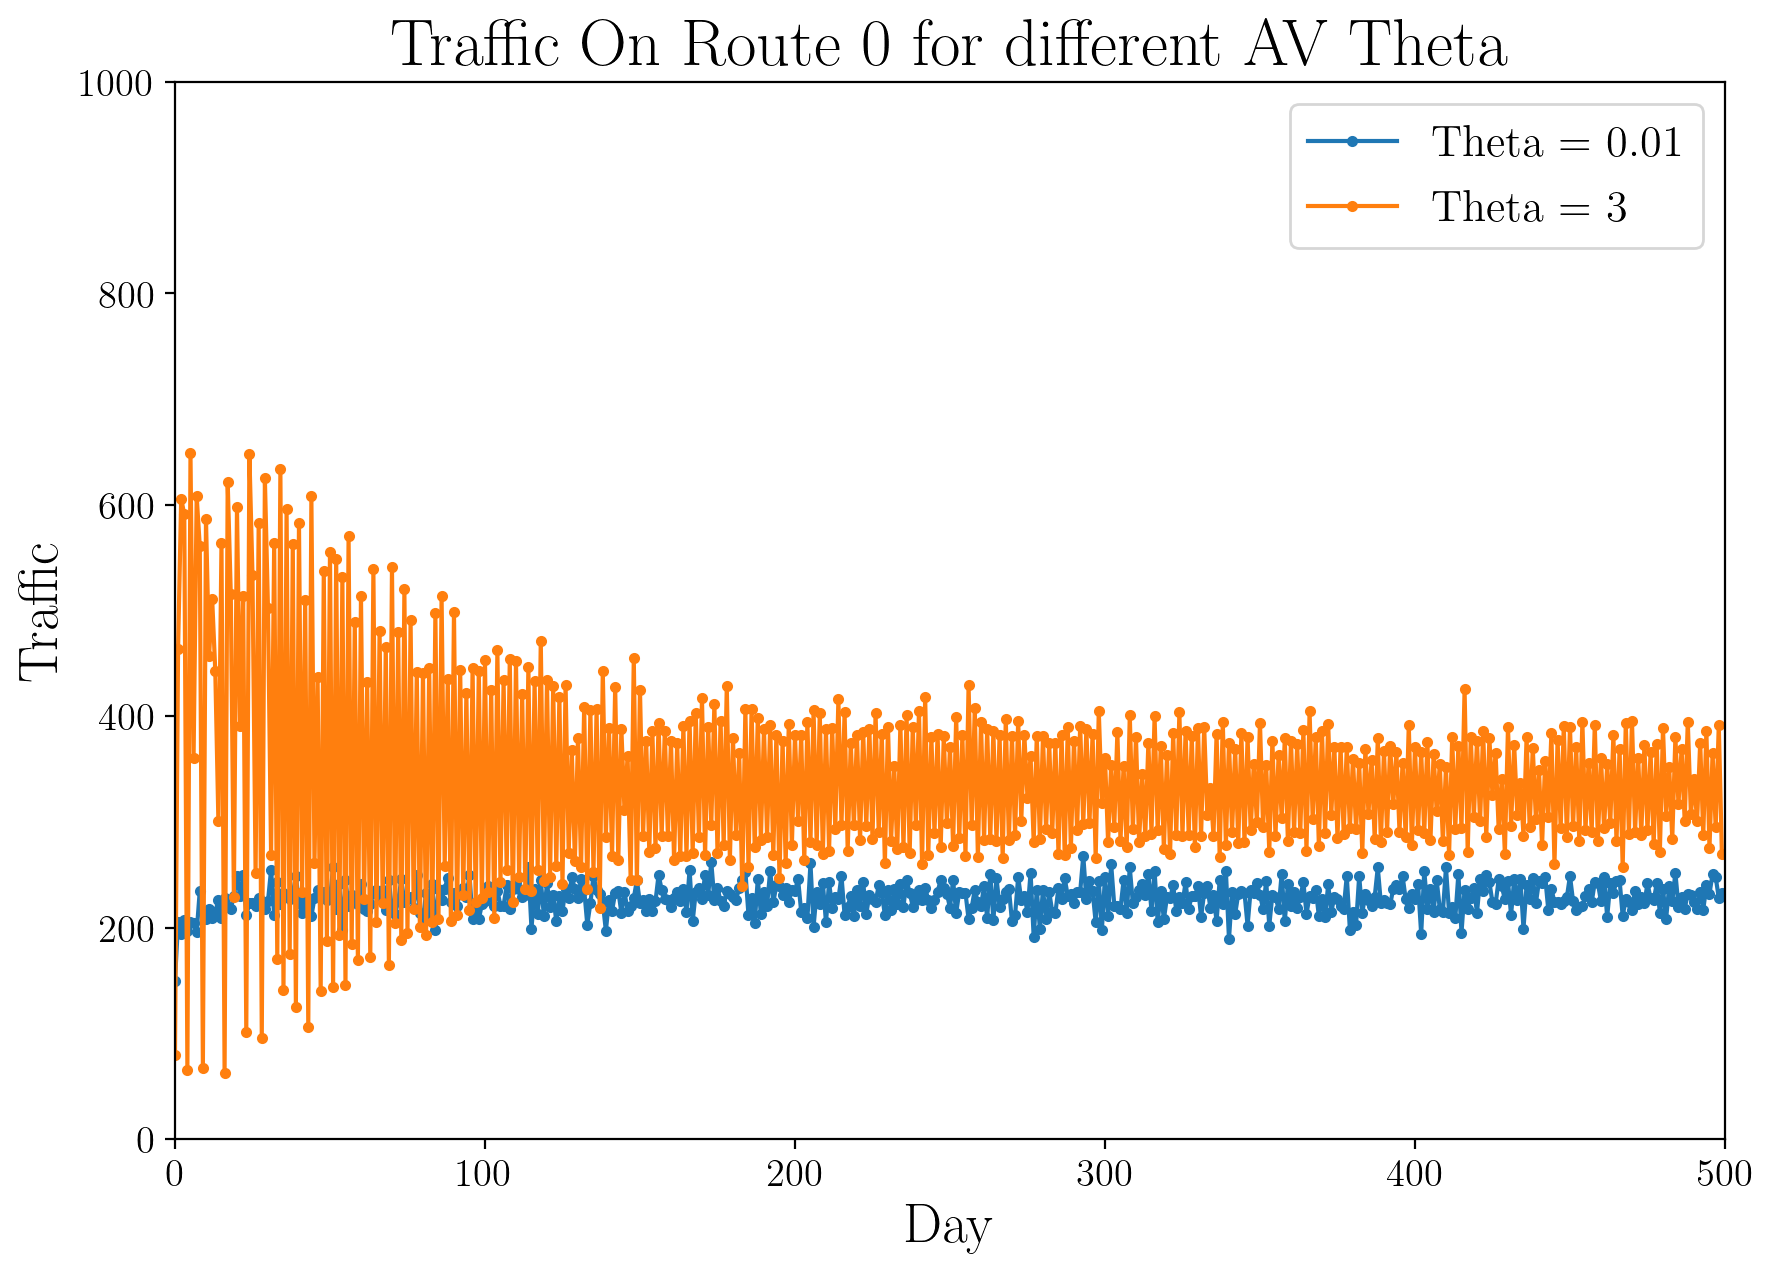
\includegraphics[scale=.5]{av_th3001_std.png}
	\caption{Results of simulations with different $\theta_{av}$}
	\label{fig:avth3001}
	\end{figure}
	
%%%%%%%%%%%%%%%%%%%%%%%%%%%%%%%%%%%%%%%%%%%%%%%%%%%%%%%%%%%%%%%%%%%%%%%%
\subsection{Effects of $L_{hv}$}
To study the effects of $L_{hv}$ the simulation was ran 10 time with the values of
$$ L_{hv} = 1, 2, 3, 4 , 10, 30, 50, 100, 250$$
with all other parameters held at their defaults.

In figure \ref{fig:hvlgrid}, four simulations are shown for references, with the traffic on routes 0 and 2 shown over the course of the simulation. In figure \ref{fig:hvlstd} the 5 day standard deviation is shown for each $L_{hv}$ value.

\begin{figure}[h!]
	\centering
	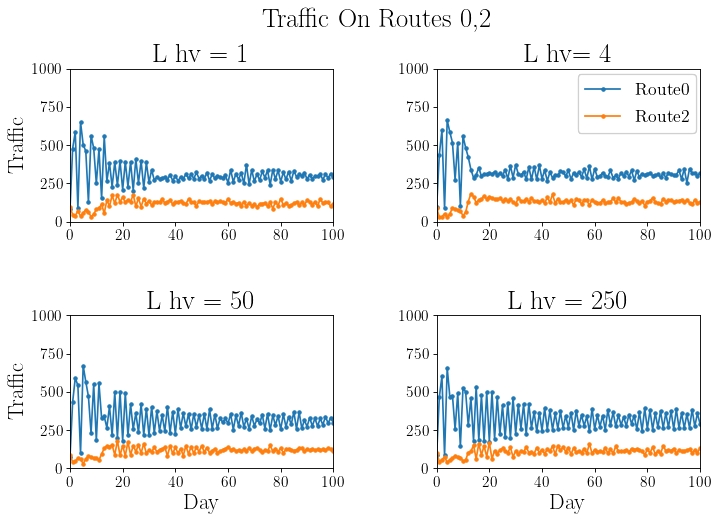
\includegraphics[scale=.5]{hv_l_grid.png}
	\caption{Results of simulations with different $L_{hv}$}
	\label{fig:hvlgrid}
	\end{figure}

\begin{figure}[h!]
	\centering
	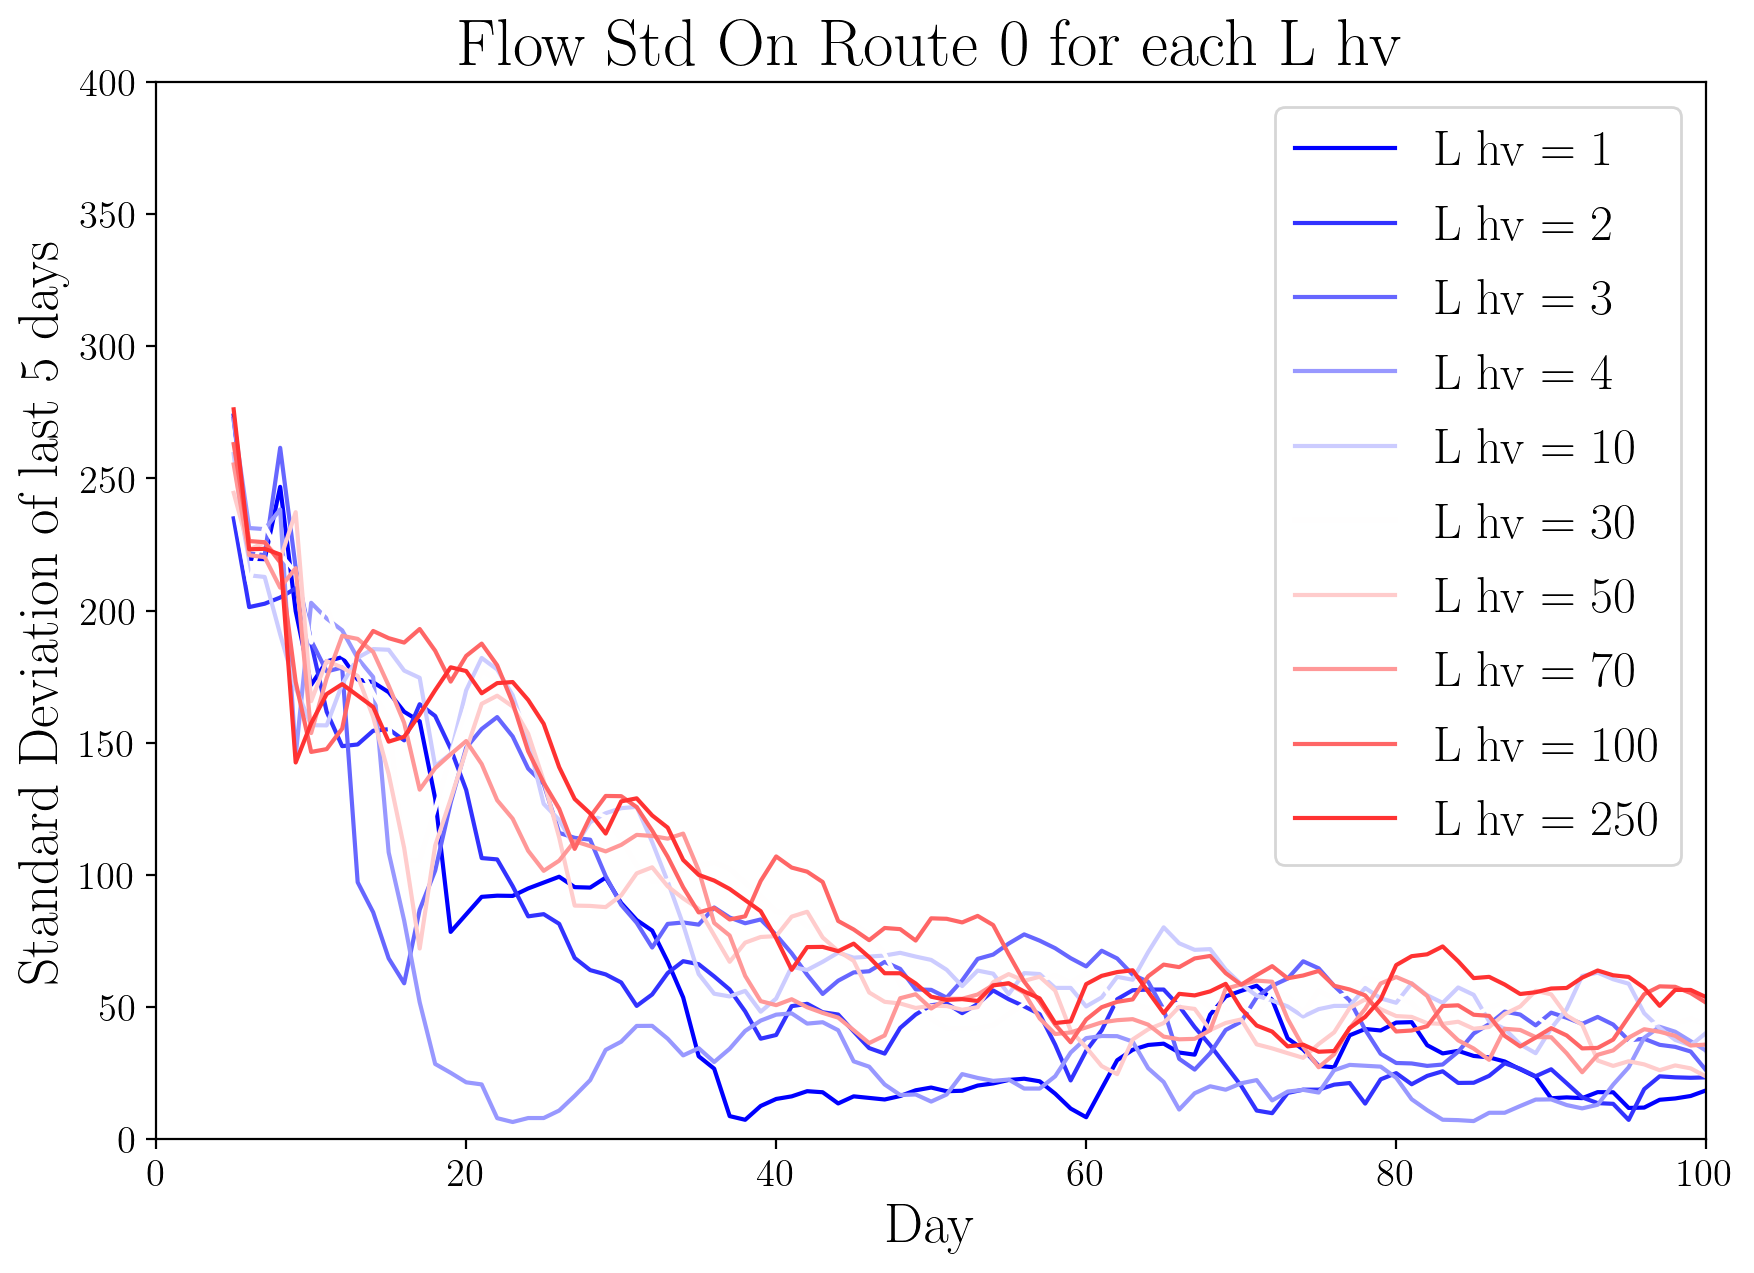
\includegraphics[scale=.5]{hv_l_std.png}
	\caption{Results of simulations with different $L_{hv}$}
	\label{fig:hvlstd}
	\end{figure}

%%%%%%%%%%%%%%%%%%%%%%%%%%%%%%%%%%%%%%%%%%%%%%%%%%%%%%%%%%%%%%%%%%%%%%%%%%
\subsection{Effects of $L_{av}$}
To study the effects of $L_{av}$ the simulation was ran 10 time with the values of
$$ L_{av} = 1, 2, 3, 4 , 10, 30, 50, 100, 250$$
with all other parameters held at their defaults.

In figure \ref{fig:avlgrid}, four simulations are shown for references, with the traffic on routes 0 and 2 shown over the course of the simulation. In figure \ref{fig:avlstd} the 5 day standard deviation is shown for each $L_{av}$ value.

\begin{figure}[h!]
	\centering
	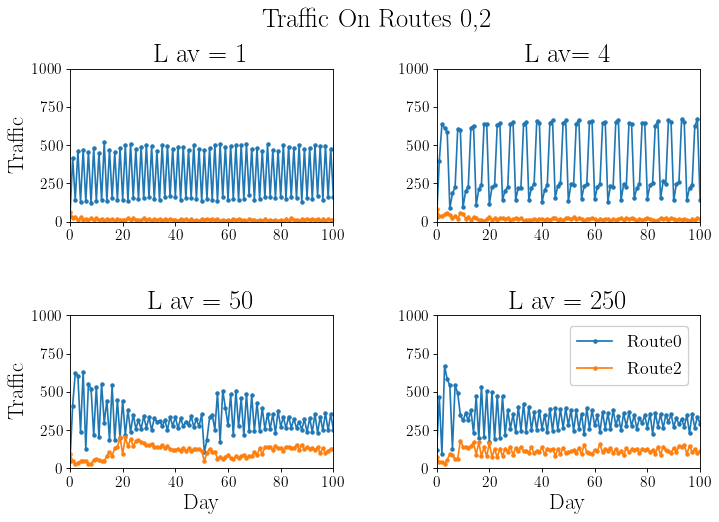
\includegraphics[scale=.5]{av_l_grid.png}
	\caption{Results of simulations with different $L_{av}$}
	\label{fig:avlgrid}
	\end{figure}

\begin{figure}[h!]
	\centering
	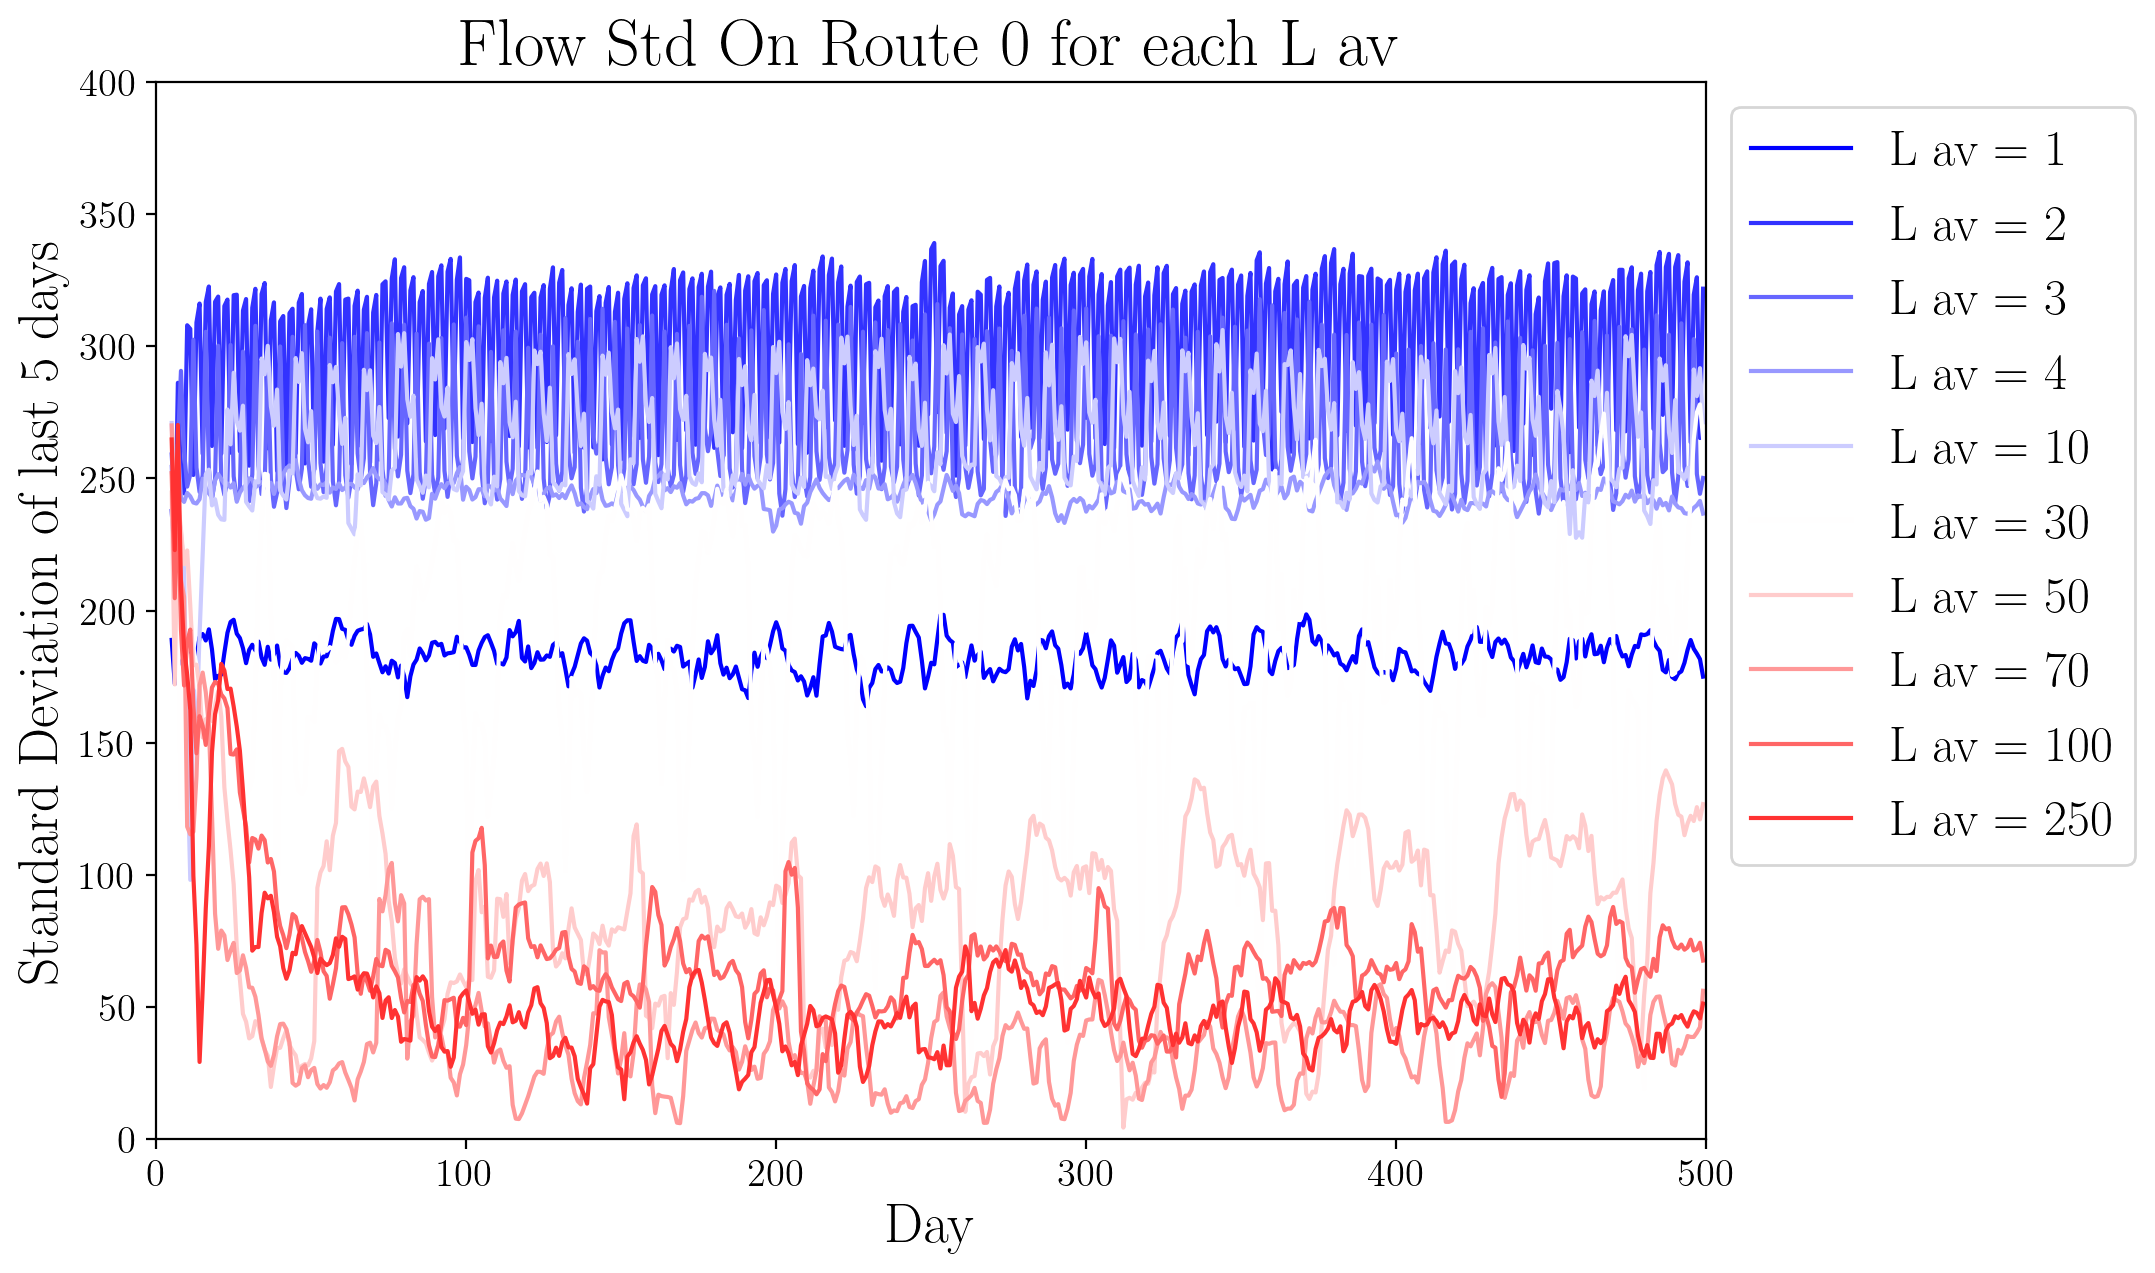
\includegraphics[scale=.5]{av_l_std.png}
	\caption{Results of simulations with different $L_{av}$}
	\label{fig:avlstd}
	\end{figure}

%%%%%%%%%%%%%%%%%%%%%%%%%%%%%%%%%%%%%%%%%%%%%%%%%%%%%%%%%%%%%%%%%%%%%%%%%%
\subsection{Effects of $\alpha$}
To study the effects of $\alpha$ the simulation was ran 10 time with the values of
$$ \alpha_{hv},\alpha_{hv} = (0,0) , (0,.5) ,(0.5,0), (.5,.5) $$
with all other parameters held at their defaults.

In figure \ref{fig:atisgrid}, all four simulations are shown for references, with the traffic on routes 0 and 2 shown over the course of the simulation.

\begin{figure}[h!]
	\centering
	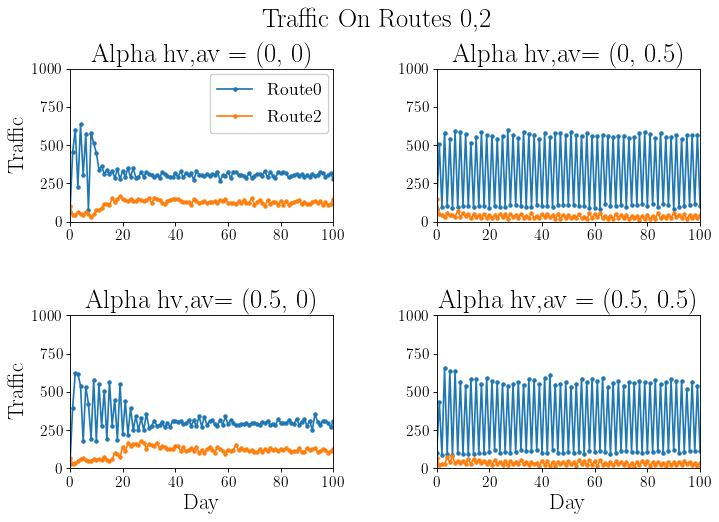
\includegraphics[scale=.5]{atis_grid.png}
	\caption{Results of simulations with different $\alpha$}
	\label{fig:atisgrid}
	\end{figure}


\pagebreak
%%%%%%%%%%%%%%%%%%%%%%%%%%%%%%%%%%%%%%%%%%%%%%%%%%%%%%%%%%%%%%%%%%%%%%%%%
% Dis
%%%%%%%%%%%%%%%%%%%%%%%%%%%%%%%%%%%%%%%%%%%%%%%%%%%%%%%%%%%%%%%%%%%%%%%%5

\section{Discussion}

\subsection{Overall Behaviour}
The model presented in this report shows consistency with models on Test Network 2 in literature.

As can be seen in figure \ref{fig:defaults} the flow on each of the six routes converged quickly, in under 100 days after which all flows remained stable around the mean of the final 250 days. They only variations visible around the mean appears to be random. This randomness is baked into the model as when a HV decided to try another route, with a probability of a half, it cannot choose the route it was on before and must explore a new route. All six routes reached equilibrium with travel times of approximately 86 seconds. 

The model is fast to run, and can be completed in 30 seconds on an Intel i7-9750H. The performance of this simulation was useful to run loops over the simulation with varying parameters, allowing for fast data collection to study the effects of the model parameters.

%%%%%%%%%%%%%%%%%%%%%%%%%%%%%%%%%%%%%%%%%%%%%%%%%%%%%%%%%%%%%%%%%%%%%%%%%%
\subsection{AV Proportion}
As can be seen in figure \ref{fig:Nhvav}, an increase in the proportion of AVs in the traffic leads to less variation and a more stable equilibrium in the long run, but not at first.

When the traffic only consists of HVs an oscillatory pattern begins to emerge as can be see in figure \ref{fig:Nhvavgrid}. The standard deviation falls quickly as each HVs build up a memory of the traffic on each route but as the simulation continues the emerging oscillatory pattern gets amplified, stabling at a higher standard deviation than when the flow first converges to the long-term means. Both the smaller standard deviation and the applied pattern center around the same means, so even as the stability lessens, the convergence values remain the same and similar to the default simulation.

One possible explanation for this is, as the memory length of each HV here is 3, an odd number, each agent will have memory in the form $(high,low,high)$ or $(low,high,low)$, with averages coming out as fairly high or fairly low. This causes the expected travel times on each route to oscillate with could explain this behaviours. This is explored in the discussion on human memory length later.

The hypnosis that memory length is causing this behaviour fits with the AV only case where the AV memory length is greater than the length of the simulation, at 1000 days. AVs see expected travel times which are the average each route has experienced so far, for all routes including once which they haven't used. This introduces stability, particularly over time as each addiction to memory will have less of an impact on the mean of the memory as the list grows. 

AVs however experience a lot of instability in the first 30 days. This could be due to a higher rationality parameter $\theta_{av}$ combined with a homogeneous memory as all agents update their memory for all routes. This would be expected to cause heavy flow on the fasted route, with all drivers agree is the most likely choice. This is explored more in the discussion on rationality. 

%%%%%%%%%%%%%%%%%%%%%%%%%%%%%%%%%%%%%%%%%%%%%%%%%%%%%%%%%%%%%%%%%%%%%%%%%%%
\subsection{Rationality}
Both the effects of $\theta_{hv}$ and $\theta_{av}$ make up the data collected to explore rationality. $\theta$ is the rationality parameter, a higher value leads to a higher probability of choosing a faster perceived route, by equation \ref{eqn:prob}.

In figure \ref{fig:hvthgrid} and figure \ref{fig:hvthstd}, convergence happens quickly over the first 20 days, then continues slower over the next 20, reaching the emergent state by day approximately 40. The standard deviation increases with $\theta_{hv}$ but not by a huge amount. Even when the rationality of the HVs is above that of the AVs they are travelling with, the convergent states are reached with only mind oscillation. 

Figure \ref{fig:avthgrid} and figure \ref{fig:avthstd} show the same experiment performed on AVs. In this case the effect is much greater. As $\theta_{av}$ increases, oscillatory behaviour develops and grows to much greater aptitudes than with the HV case. Flow over all routes when $\theta_{av} = 0.01$ is particularly stable, although it does appear to be at a lower level. By calculating the average of the final 250 days on route 0 ,the convergence point is found be $228.0$, below the default case of 305.2. In the cases of low $\theta_{av}$ convergence also happens significantly faster than the default case.

When $\theta_{av} = 3$ the traffic on route 0 takes nearly 200 days to converge, and shows high amplitude random oscillations around a higher mean of 341.4. Due to the homogeneous memory of AVs, it is expected that higher rationality would cause too much traffic on the fasted routes, and route 0 is the fastest in free flow. This would explain the traffic on route 0 but not the oscillatory behaviour.

It is clear that overly rational AVs may lead to worse traffic, without more intelligent decision making algorithms that understand these effects and attempt to prevent them. 

%%%%%%%%%%%%%%%%%%%%%%%%%%%%%%%%%%%%%%%%%%%%%%%%%%%%%%%%%%%%%%%%%%%%%%%%%%
\subsection{Memory}
Figure \ref{fig:hvlgrid} shows the results when HV memory is 1, 4, 50, and 250, while figure \ref{fig:hvlstd} shows the effects memory length has on the standard deviation. 

The standard deviations suggest HV memory length does not have a huge impact on convergence speed, with lower shorter values of $L_{hv}$ converging slightly faster higher ones. Higher $L{hv}$ also have a higher standard deviation once a steady state has been reached. The hypnosis that the odd values of $3$ for $L_{hv}$ was causing oscillatory behaviour seem not to hold, as oscillatory behaviour continues to be seen as is highlighted in figure \ref{fig:hvlgrid} for $L_{hv} = 4$.

The effects of memory for AVs is drastic. In figure \ref{fig:avlgrid} it can be seen that small memory lengths lead to high amplitude oscillatory behaviour. The $L_{av}$ case appears to show a approximately stable 5-cycle. This could be due to agents forgetting the travel times from 5 days ago causing them to repeat themselves. Agents with homogeneous memory appear to need complete memory in order to stabilise without oscillations.

To test this an extra simulation was ran with $L_{av} = 4$ and $N_{av} = 1000$ with no HVs. A portion on the results showing the traffic on route 0 on between day 20 and day 40 is shown in \ref{fig:avlextra}.

\begin{figure}[h!]
	\centering
	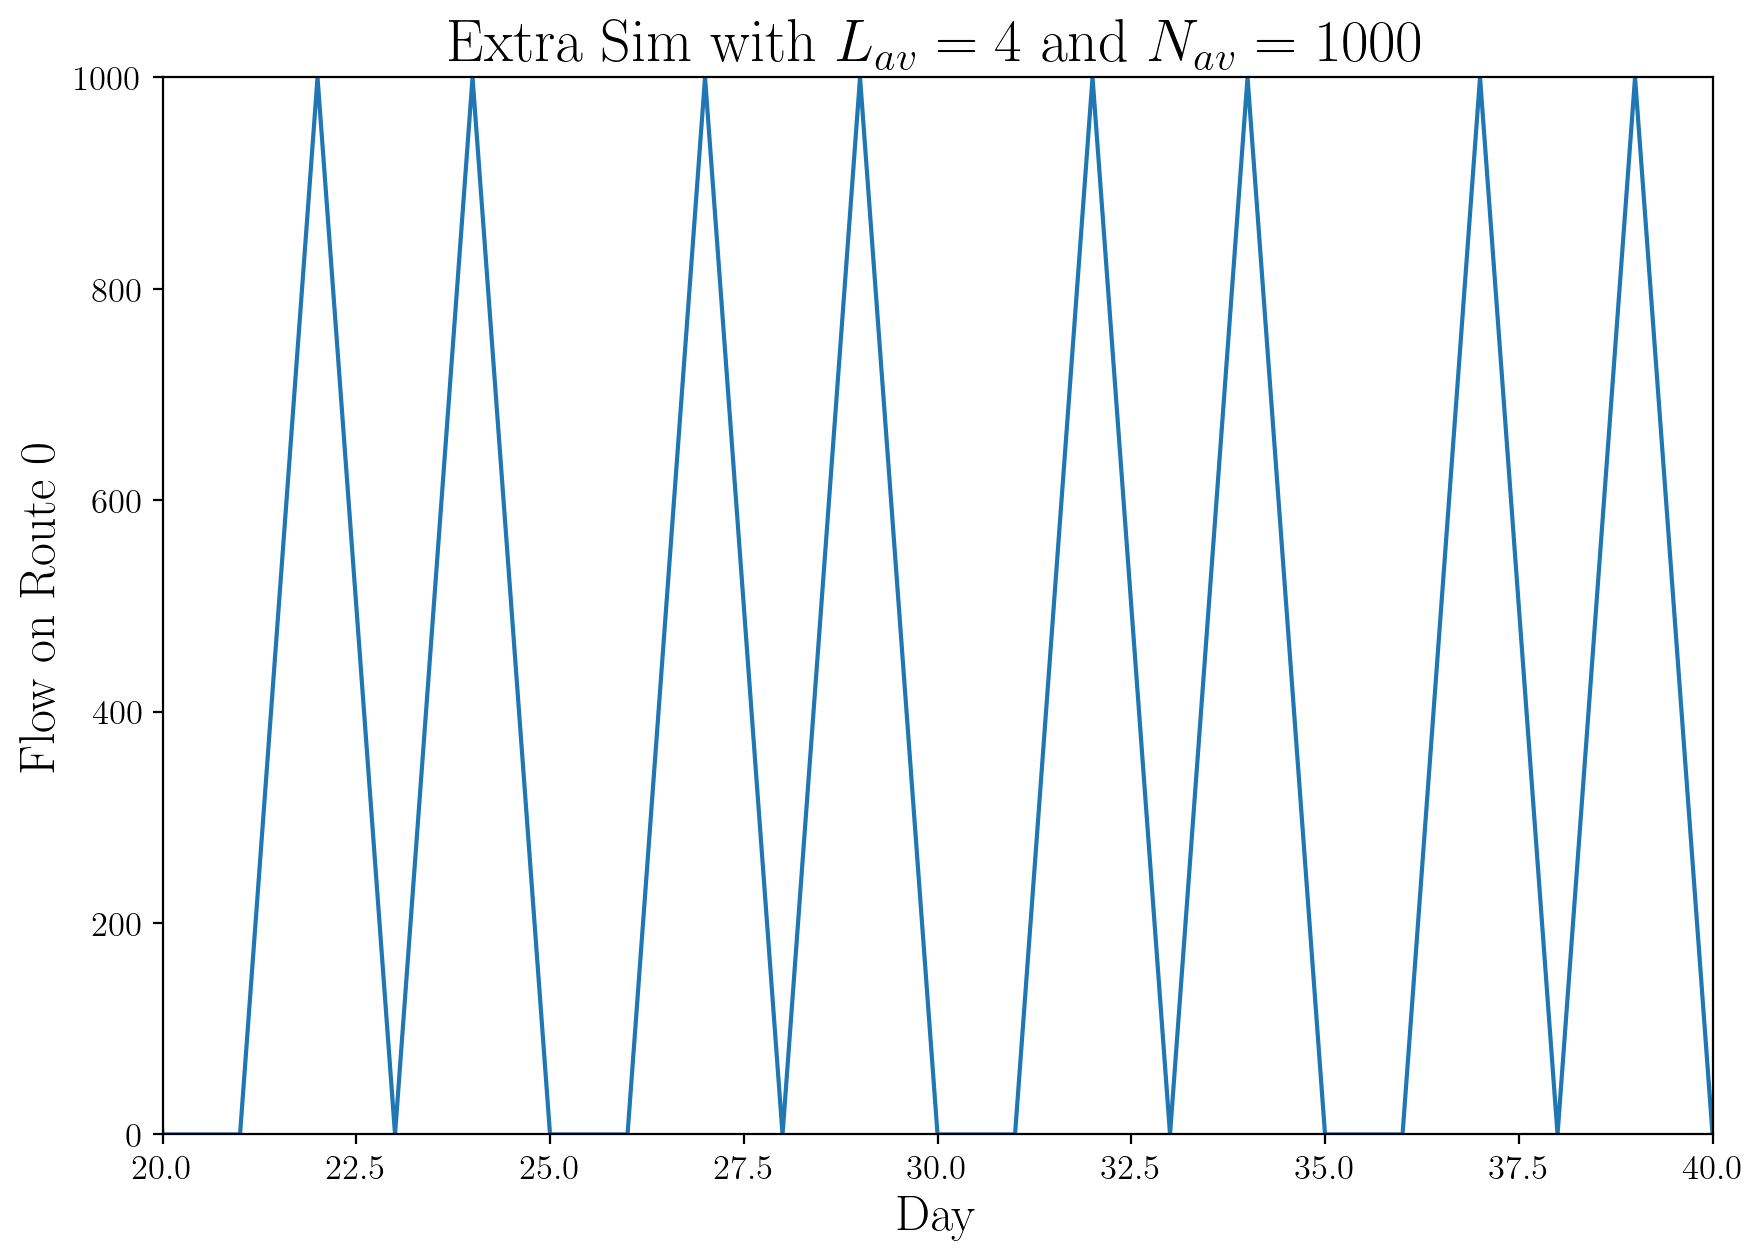
\includegraphics[scale=.5]{av_l_extra.png}
	\caption{Section of results from extra simulation on $L_{av} = 4$, results between days 20, and 40}
	\label{fig:avlextra}
	\end{figure}

Memory can also include information from the the Advanced Traveller Information System. The ATIS mixes the previous days information for all routes with the agents memory. This could have the effect of \textit{blending} the sort memory length case with the longer case. 

From studying figure \ref{fig:atisgrid} it can be seen the the ATIS has small difference to HVs but causes high amplitude oscillations in AVS. This agrees with the hypnosis of blending cases. The small effect on HVs is likely due to their short memory, so blending $L_{hv} = 4$ and $1$ makes no difference, however the ATIS causes HVS con convergence much slower, taking approximately 40 days instead of 20.

\subsection{Comparison With Literature}
Comparing with literature, in \cite{Wei2014} it was found that longer memory led to more stability, however in their model memory was a weighted average of past experiences. The HV case in this report's model disagrees with this, with higher $L_{hv}$ leading to more oscillations. The AV case agrees with the literature as a better memory leads to better convergence and less oscillation.

Although this report's model has no learning rate, $l$ from \cite{Wei2014} can be thought of as a rationality parameter. Both the AV and HV cases agree with their results as higher rationality leads to less stable steady states and more oscillation. 

The simple ATIS in this report's model shown that providing HVs with accurate information does make flow convergence occur slower, but it still converges, unlike the oscillatory pattern found by \cite{Liu2007}. AVs already have access to accurate information as they have no error. However the ATIS prevents AVS from using their average travel times and instead favours the previous days tims, this causes powerfully oscillations and the instability found in \cite{Liu2007}.

%%%%%%%%%%%%%%%%%%%%%%%%%%%%%%%%%%%%%%%%%%%%%%%%%%%%%%%%%%%%%%%%%%%%%%%%%%
% Conclusions
%%%%%%%%%%%%%%%%%%%%%%%%%%%%%%%%%%%%%%%%%%%%%%%%%%%%%%%%%%%%%%%%%%%%%%%%%%

\section{Conclusions}
From the Simulations and analysis in this report, it can be seen that autonomous vehicles could improve traffic flow but only when implemented correctly.

An agent based model was built with separate human and autonomous vehicles. HVs chose a route based on their memory from experiences while AVS learned from collective experience. Humans had error in their perception while AVs did not. Agents chose a route with a higher probability for faster routes, with AVs preferring faster routes more than HVs. 

The agents drove on a grid network from a common origin to a common destination. They had choice of routes which shared links with each other. They began with vague knowledge of travel times, with a lot of error, and learned from experience. They drove 500 times, learning every time.

Introducing AVs does lead to initial instability, which get worse as AV penetration gets higher, but this is only initial as the AVs \textit{learn} the network. Higher AV penetration does improve travel times towards the end of the simulation. In reality when AVs are deployed, they will likely already have access to information, and a gradual introduction should not lead to the instability seen as the simulation begins. 

It is also clear that for AVs to mix well with humans, \textit{artificial irrationally} could be extremely useful. By limiting the information available to the AVs while choosing a route, and preventing them all from choosing the fastest route, the traffic will spread out more evenly. 

Preventing overcrowding on fast routes will be one of the important tasks to master when developing autonomous vehicles, but performed successfully could lead to improved travel times for all road users.




%%%%%%%%%%%%%%%%%%%%%%%%%%%%%%%%%%%%%%%%%%%%%%%%%%%%%%%%%%%%%%%%%%%%%%%%%
% Append
%%%%%%%%%%%%%%%%%%%%%%%%%%%%%%%%%%%%%%%%%%%%%%%%%%%%%%%%%%%%%%%%%%%%%%%%%
\pagebreak
\bibliography{final}


\pagebreak
\section*{Appendix A: Python Code}
\addcontentsline{toc}{section}{Appendix 1: Python Code}

\subsection*{Simulation Script}
\lstinputlisting{../final/sim_script_demo.py}

\pagebreak
\subsection*{Agent Module}
\lstinputlisting{../final/agents.py}

\pagebreak
\subsection*{Environment Module}
\lstinputlisting{../final/environment.py}


\pagebreak
\section*{Appendix B: Gantt Chart}
\addcontentsline{toc}{section}{Appendix 2: Gantt Chart}

\begin{figure}[h!]
	\centering
	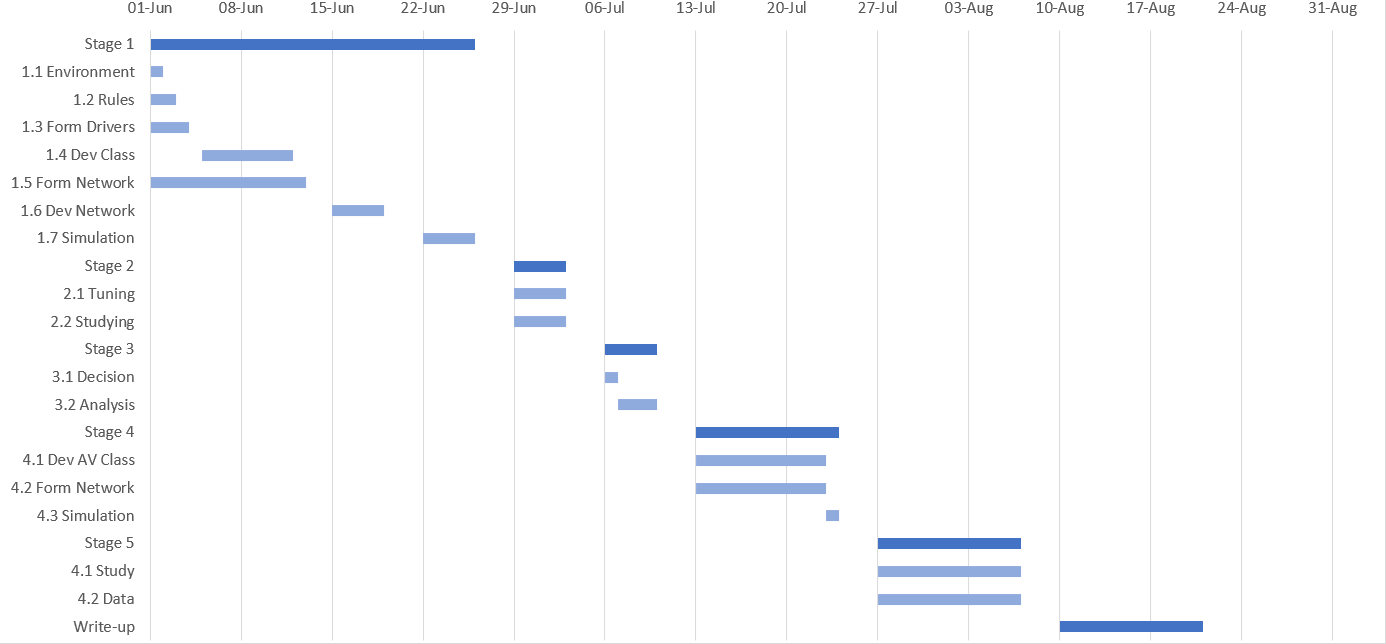
\includegraphics[scale=.65, angle = 90]{gantt.png}
	\end{figure}


\end{document}
